\setcounter{chapter}{1}

\chapter{数列极限与数值级数}

\section{数列极限}

\subsection{数列}

{\bf 教材:}按一定规律排列的无穷多个(相同或不相同的)数,记作:
\ps{\b 有序性是数列最重要的特征,改变了数列中数的排列顺序将得到不同的数列}
$$a_1,a_2,\ldots,a_n,\ldots$$
或者$\{a_n\}$。

$\{a_n\}$的实质是定义在$\mathbb{N}_+$上的函数,即所谓的{\it 整标函数}或{\it 整序函数}
\ps{教材上的说法是“可视为”},即
$$a_n:\mathbb{N}_+\mapsto\mathbb{R}$$

如果在平面直角坐标系内作图,也可以将其视为一个动点随$n$增大所留下的运动轨迹。

{\bf 思考:}数列与集合有哪些区别?\ps{1、有序-无序;\\ 2、无限-可能有限;\\ 3、可重复-不可重复}

{\bf 例:}数列举例

\begin{enumerate}[(1)]
  \setlength{\itemindent}{1cm}
  \item[(1)] $\left\{\df{n+1}n\right\}:\df 21,\df 32,\df43,\df54,\df65,\ldots$
  \item[(2)] $\left\{\df{(-1)^n}n\right\}:-1,\df12,-\df13,\df14,-\df15,\df16,\ldots$
  \item[(3)] $\{n^2\}:1,4,9,16,25,36,\ldots$
  \item[(4)] $\left\{n^{(-1)^n}\right\}:1,2,\df13,4,\df15,6,\ldots$
\end{enumerate}

\subsection{数列的极限}

{\bf 极限:}$a_n$的值随$n$的不断增大而趋向的稳定的值
\ps{现实生活里的极限更类似于我们所说的上限(确界)和下限(确界),例如:人类速度的极限} 

{\bf 例:}(1)$\limn\df1n=0$;\quad(2)$\limn\df{n^2}{n^2-1}=1$;
\quad(3)$\limn\sqrt[n]2=1$

\bigskip

本节我们主要关注一个问题:{\it 数学上如何表达这种趋向某个稳定值的特征,或者说,
给出数列极限的数学定义。}

{\bf 定义:}对于数列$\{a_n\}$,若存在常数$a$,{\b 对任意$\e>0$,
均存在$N\in\mathbb{Z}_+$,
% \ps{\b 教材上强调$N\in\mathbb{Z}_+$,其实是完全没有必要的}
对任意$n>N$,恒有
$$|a_n-a|<\e$$
成立},则称{\it 数列$\{a_n\}$存在极限(或收敛)},常数$a$称为该数列的极限,记为
$$\lim_{n\to\infty}a_n=a$$
或\ps{\b 使用后面一种记号时,必须要写上$(n\to\infty)$}
$${\b a_n\to a\;(n\to\infty)}$$
若上述常数$a$不存在,则称数列$\{a_n\}$不存在极限(或{\bf 发散})。

从几何上看(如下图所示),数列$\{a_n\}$以$a$为极限,意味着随着$n$的增大,$a_n$可以无限地
靠近$a$。为了表达这种“无限靠近”,数学上可以这样来解释:对于以$a$为中心的任意小的邻域$(a-\e,
a+\e)$(图上的蓝色阴影部分),只要把$n$取得充分大($N$的意义就是为了界定这个所谓的充分大$^{\b (1)}$),
\ps{\b (1)显然,$\e$取得越小通常意味着$N$要取得越大,但必须注意的是$N$和$\e$之间并不是简单的函数对应
关系,因为如果某个$N$可以满足命题要求,则$N$加任意的正常数显然也满足}
则$a_n$都将落在$(a-\e,a+\e)$之内$^{\b (2)}$
\ps{\b (2)除了有限多个$a_n$外(准确地说是除了至多$\{a_n\}$的前$N$项外)}

\begin{center}
	\resizebox{!}{3cm}{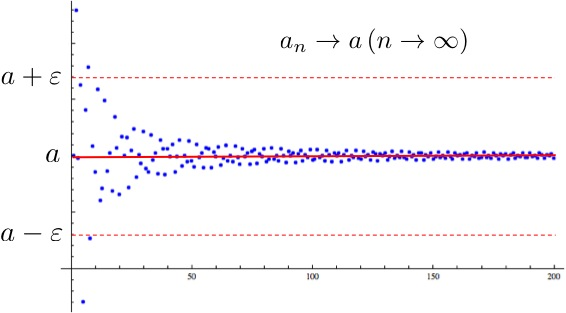
\includegraphics{./images/ch2/lim-en/en1.jpg}}\quad
	\resizebox{!}{3cm}{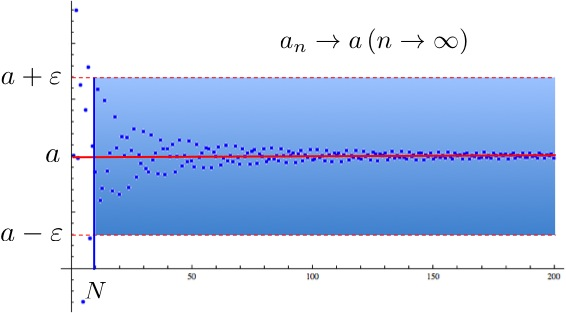
\includegraphics{./images/ch2/lim-en/en2.jpg}}
	
	\resizebox{!}{3cm}{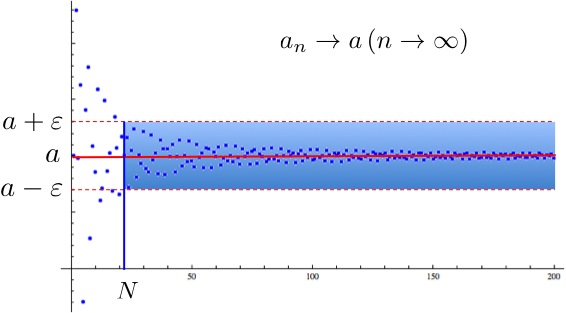
\includegraphics{./images/ch2/lim-en/en3.jpg}}\quad
	\resizebox{!}{3cm}{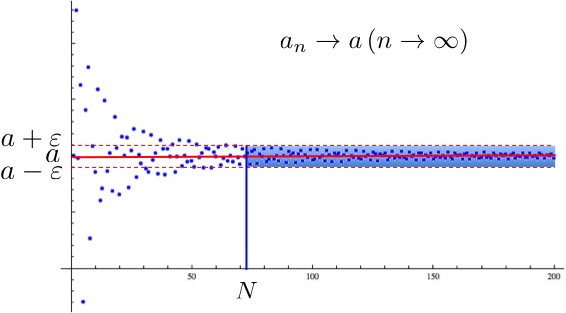
\includegraphics{./images/ch2/lim-en/en4.jpg}}
	
	\resizebox{!}{3cm}{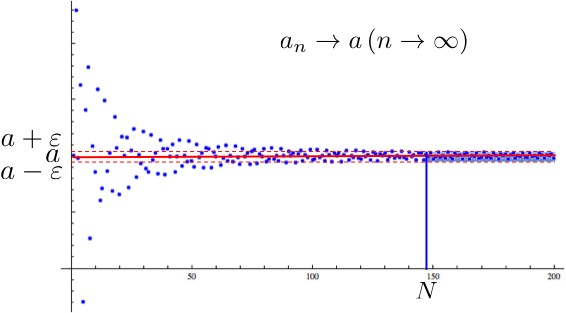
\includegraphics{./images/ch2/lim-en/en5.jpg}}
\end{center}

前述定义更为简洁的写法:\ps{这种纯符号的表述方式固然简洁,但要正确掌握,
必须首先对更完整的文字表述有准确的理解,否则不建议随意使用}

$$%\lim_{n\to\infty}a_n=a\quad\Leftrightarrow\quad
{\b \forall\e>0,\exists N\in\mathbb{Z}_+,\forall n>N,|a_n-a|<\e}\eqno{(1)}$$

{\bf 讨论:}以下说法和$(1)$等价的是:

\begin{enumerate}
  \setlength{\itemindent}{1cm}
%   \item[(2)] $\forall\e>0$,$\exists N>0$,$\forall
%   n>N$,$|a_n-a|<\e$ \hfill{$\surd$}\\
%   \hfill(直接写$\exists N$即可)
  \item[(2)] $\forall\e>0$,$\exists N$,$\forall
  n>N$,$|a_n-a|\leq\e$ \hfill{$\surd$} 
  
  {\quad 注:只要强调$n>N$为正整数即可,根据需要$N$总是可以取得更大,无所谓是不是正整数}
  \item[(3)] $\exists N\in\mathbb{Z}_+$,$\forall\e>0$,$\forall
  n>N$,$|a_n-a|<\e$ \hfill{$\times$}
  
  {\quad 注:(3)$\Rightarrow$(1),反之不然。事实上,由(3)可以推出,
  $\{a_n\}$仅有有限项的值不等于$a$}
  \item[(4)] $\forall\e>0$,仅有有限多个$n$,使得$|a_n-a|\geq\e$
  \hfill{$\surd$}
 
  \item[(5)] $\forall\e>0$,总有无穷多个$n$,使得$|a_n-a|<\e$
  \hfill{$\times$} 
  
  {\quad 反例:$a_n=(-1)^n$,取$a=1$}
  \item[(6)] $\forall\e>0$,要使$|a_n-a|<\e$,只须$n$充分大 \hfill{$\surd$}
  
  {\quad 注:等价,语序有变化,但逻辑关系未发生改变}
  \item[(7)] $\forall\e>0,\exists N\in\mathbb{Z}_+,\forall
  n>N,|a_n-a|<2\e$\hfill{$\surd$}
  
  {\quad\b 注:注意到$\e$是任意的,$2\e$和$\e$的取值范围并没有区别!事实上,$2\e$
  完全可以改成$C\e$,其中$C\in\mathbb{R}$为给定的常数。今后在用定义证明极限时,我们
  常常使用该命题作为定义的等价说法}
\end{enumerate}

% {\bf 注:}
% 
% \begin{itemize}
%   \setlength{\itemindent}{1cm}
%   \item $a$是确定的数 ( {不能是$\pm\infty$}) 
%   \item “$\forall\e>0$”应该理解为{“对任意小的$\e>0$”}
%   \item $N$由$\{a_n\}$和$\e$共同决定, “存在$N$”可理解为{“存在充分大的$N(\e)$}”; 
%    {如果$N$能够满足定义, 任意比$N$大的数都能够满足定义; 通常$\e$取得越小,
%   $N$需要取得越大} \ps{$\{a_n\}$的收敛性与其任意多的有限项无关!!}
%   \item 给定$C>0$,“$|a_n-a|<\e$” 可替换为{“$|a_n-a|<C\e$”}, 其中$C>0$为常数
% \end{itemize}

{\bf 例:}证明:
$$\limn(-1)^n\df1{n^2}=0$$

{\bf 证:}对任意$\e>0$,{\b 令$N=\left[1/\sqrt{\e}\right]+1$}
\ps{不要忘记:\b $[x]\leq x<[x]+1$}
,则对任意$n>N$,有
$$\left|(-1)^n\df1{n^2}-0\right|=\df1{n^2}<\df1{N^2}=\e,$$
由极限的定义,即证。\ps{\b 用定义证明数列极限,说明$N$的存在性是关键,为此主要有两种方式:\\
(1)直接给出$N$的取值,例如$N=1/\e$\\
(2)利用已知极限间接说明$N$存在,如$N=N_1$}

{\bf 例:}证明:
$$\limn\left(\df n{n+1}\right)^2=1$$

{\bf 证:}对任意$\e>0$,{\b 令$N=\left[2/\e\right]+1$},则对任意$n>N$,有
$$\left|\left(\df
n{n+1}\right)^2-1\right|=\df{2n+1}{(n+1)^2}<\df{2(n+1)}{(n+1)^2}
<\df2{n+1}<\df2n<\df2N=\e,$$
由极限的定义,即证。

{\bf 例:}证明:若$\limn a_n=a$,则$\limn|a_n|=|a|$

{\bf 证:}对任意$\e>0$,由$\limn a_n=a$可知,存在$N_1\in\mathbb{Z}_+$,
对任意$n>N_1$,有
$$|a_n-a|<\e.$$
于是{\b 令$N=N_1$},则对任意$n>N$,有\ps{\b 利用$N_1$的存在性间接说明了$N$的存在性}
$$||a_n|-|a||\leq|a_n-a|<\e,$$
由极限的定义,即证。

{\bf 课堂练习:}证明:若$|q|<1$,则$\{q^n\}$收敛。

[提示]:令$N=\left[\log_{|q|}\e\right]+1$

% {\bf 思考:}已知$|q|>1$时,$\{q^n\}$发散,请问该如何证明?
% 
% {\bf 注:}利用有界性,也可以证明发散。

\begin{shaded}
	{\bf 【极限定义的反面说法】}
	
	$$\limn a_n\neq a\quad\Leftrightarrow\quad\exists\e_0>0,
	\forall N\in\mathbb{Z}_+,\exists n_0>N,|a_{n_0}-a|\geq\e_0$$
	
	{\bf 例:}证明:$\limn\df 1n\neq 1$
	
	{\bf 证:}取$\e=\df12$,对任意$N\in\mathbb{Z}_+$,令$n_0=\max\{3,[N]+1\}>N$,
	从而
	$$\left|\df1{n_0}-1\right|=1-\df1{n_0}\geq 1-\df13=\df23>\e,$$
	由极限的反面定义,即证。
	
	{\bf 教材2.1.2节-例5:}证明$\{(-1)^n\}$发散。
	
	{\bf 证:}任取$a\in\mathbb{R}$,只需证明$\limn(-1)^n\ne a$。以下不妨设$a>0$。
	
	取$\e=1$,对任意$N\in\mathbb{Z}_+$,令$n_0=\max\{2[N]+1,1\}>N$,则
	$$\left|(-1)^{n_0}-a\right|=|-1-a|=a+1>\e,$$
	由极限的反面定义,即证。
	
	{\bf 注:}相对于教材上所使用的反证法,用反面定义证明极限不存在,形式上更简洁,但
	却不是特别直观和容易理解。
	
	{\bf 思考:}数列发散可能有哪些不同的情形?({\it 趋向无穷,或反复振荡})
	
\end{shaded}

\subsection{数列极限的基本性质}

\subsubsection{【唯一性】}

{\bf 定理2.1.1:}数列极限若存在,必唯一。\ps{唯一性的要求决定了当前的极限定义。
从这个意义上说,目前使用的极限定义其实也是一种约定。}
%“记录重大技术突破的技术发展史其实就是一部人类社会发展的技术选择史”

\begin{center}
	\resizebox{!}{4cm}{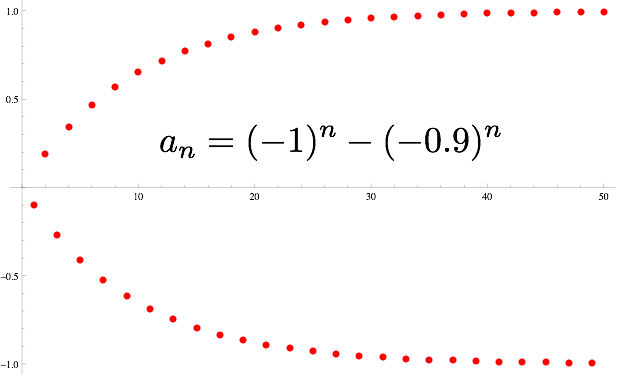
\includegraphics{./images/ch2/1-0.9n.jpg}}
\end{center}

{\bf 引理:}{\b 设$a,b\in\mathbb{R}$,若对任意$\e>0$,有$|a-b|<\e$,则$a=b$}
\ps{\b 两个确定的数如果可以无限靠近,则意味着它们相等。}

定理证明请自行阅读教材。

{\bf 定理证明:}设$a,b$均为数列$\{a_n\}$的极限,$a\ne b$。

对任意$\e>0$,由$\limn a_n=a$,存在$N_1\in\mathbb{Z}_+$,对任意$n>N_1$,有$|a_n-a|<\e$;
同理,由$\limn a_n=b$,存在$N_2\in\mathbb{Z}_+$,对任意$n>N_2$,有$|a_n-b|<\e$。

令{\b $N=\max\{N_1,N_2\}$},则当$n>N$时,有
$${\b |a-b|\leq|a_n-a|+|a_n-b|<2\e},$$
由此可知,必有$a=b$,与假设矛盾,即证。

\subsubsection{【有界性】}

{\bf 定理2.1.2:}数列$\{a_n\}$若收敛,则$\{a_n\}$必有界,即存在$M>0$,对任意
$n\in\mathbb{Z}_+$,恒有$|a_n|\leq M$。

\begin{center}
	\resizebox{!}{4cm}{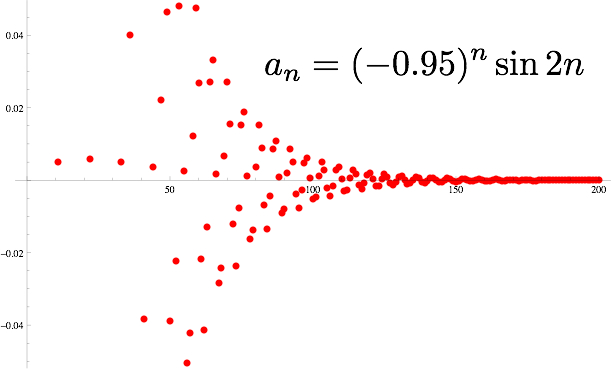
\includegraphics{./images/ch2/sin2nn.jpg}}
\end{center}

{\bf 思路:}{\b 利用$\e$的特定取值控制无穷的部分,剩余的有限多个数构成的集合自然是有界的}

{\bf 证:}记$\limn a_n=a$。由极限的定义,对{\b$\e=1$},存在$N\in\mathbb{Z}_+$,对任意$n>N$,有
$$|a_n-a|<\e=1\quad\Rightarrow\quad |a_n|<|a|+1.$$
记{\b$M=\max\{|a|+1,|a_1|,|a_2|,\ldots,|a_{[N]+1}|\}$},则对任意$n\in\mathbb{Z}_+$,
均有
$$|a_n|\leq M,$$
即证。

{\bf 例:}讨论$\{\sqrt[n]{n!}\}$的敛散性。

[提示]:任意$M>0$,当$n$充分大时,总有$n!>M^n$,故$\{\sqrt[n]{n!}\}$无界,
从而发散。\ps{\b 证明数列无界,是证明其发散的一种典型方法}

{\bf 证:}对任意$M>0$,令$N=[2M]+1$,则当$n>N$时,总有$n>2M$。此时
$$\df{n!}{M^n}=\df{N!}{M^N}\cdot\df{N+1}{M}
\cdot\df{N+2}{M}\ldots\df{n}{M}<\df{N!}{M^N}\cdot2^{n-N+1}.$$
注意到$\df{N!}{M^N}$为有限值,而$2^{n-N+1}$随着$n$的增大趋于正无穷,
故当$n$充分大时,必有
$$\df{n!}{M^n}=\df{N!}{M^N}\cdot2^{n-N+1}>1,$$
从而$\sqrt[n]{n!}>M$,由此即证$\{\sqrt[n]{n!}\}$无界,从而发散。

\subsubsection{【保号性】}

{\bf 定理2.1.3:}设$\lim\limits_{n\to\infty}a_n=a>0$,则存在$N$,
对任意$n>N$,$a_n>0$

{\bf 证:}由$\lim\limits_{n\to\infty}a_n=a>0$,对$\e=a/2$,存在
$N$,对任意$n>N$,
$$|a_n-a|<\e=a/2\quad\Rightarrow\quad \df32a>a_n>a/2>0,$$
即证。
		
{{\bf 推论:}} 
\begin{enumerate}
  \setlength{\itemindent}{1cm}
  \item {\b 对任意$n\in\mathbb{N}$,$a_n\geq
  0$, $\lim\limits_{n\to\infty}a_n=a$, 则$a\geq 0$}
%   \ps{\b 保号性可以理解为极限运算保持不等号的方法不变,即:由$a_n\geq 0$
%   可推出$\limn a_n\geq0$} 
  \item {\b 设$\lim\limits_{n\to\infty}a_n=a\ne
  0$, 则$\exists N$,当$n>N$时,$|a_n|>|a|/2$} 
  \item {\b 
  设$\lim\limits_{n\to\infty}a_n=a$, 且最多有有限个$a_n$小于零, 则$a\geq 0$}
\end{enumerate}	

{\bf 注:}{\b 保号性的实质,是极限运算保持不等号的方向不变
$$a_n\geq b_n\,(n\in\mathbb{Z}_+)\quad\Rightarrow
\quad\limn a_n\geq\limn b_n$$
}

\section{数列极限的性质与判敛}

\subsection{四则运算的性质}

{\bf 定理2.2.1:}
设数列$\{a_n\},\{b_n\}$分别以$a,b(b\neq 0)$为极限,则
数列$\{a_n\pm b_n\},\{a_nb_n\},\left\{\df{a_n}{b_n}\right\}$均收敛,且
\begin{enumerate}
  \setlength{\itemindent}{1cm}
  \item $\limn(a_n\pm b_n)=a\pm b$
  \item $\limn a_nb_n=ab$
  \item $\limn\df{a_n}{b_n}=\df ab$
\end{enumerate}

{\bf 注:}{\b 极限运算和四则运算可以交换次序——前提是
所有相关的极限均存在,且为有限次四则运算}

{\bf 注意:}{\b 典型错误
\begin{eqnarray*}
	1&=&\limn \underbrace{\left(\df 1n+\df 1n+\cdots+\df 1n\right)}_{n}\\
	&=&\underbrace{\limn\df1n+\limn\df1n+\cdots+\limn\df1n}_{n}\\
	&=&n\limn\df1n=0
\end{eqnarray*}}
相当于$n$落在了极限符号之外,显然错误!!

{\bf 教材2.2.1节-例2:}计算极限
$$\limn\df{2n^6+3n^4-n+10}{n^6+n^4+1}$$

{\bf 解:}
\begin{align}
	\mbox{原式}&=\limn\df{2+3\df1{n^2}-\df1{n^5}+10\df1{n^6}}
	{1+\df1{n^2}+\df1{n^6}}\notag\\
	&=\limn\df{2+3\limn\df1{n^2}-\limn\df1{n^5}+10\limn\df1{n^6}}
	{1+\limn\df1{n^2}+\limn\df1{n^6}}=2\notag
\end{align}

{\bf 注:}{\b 对于有理函数列求极限,可以参照如下公式计算(设:$s,t\in\mathbb{Z}_+,a_s\cdot b_t\ne 0$)
$$\limn\df{\sum\limits_{i=1}^s a_in^i}{\sum\limits_{i=1}^t b_in^i}
=\left\{\begin{array}{ll}
\mbox{发散},& s>t\\
0,&s<t\\
\df{a_s}{b_t},&s=t
\end{array}\right.$$}

% {\bf P58-例1:}设$\limn(a_n+b_n)=1$,$\limn(a_n-b_n)=3$,证明$\{a_n\},\{b_n\}$收敛,并求其值。

{\bf 例:}计算极限
$$\limn\df{\cos^n\theta-\sin^n\theta}{\cos^n\theta+\sin^n\theta}\quad
(0\leq\theta\leq\df{\pi}{2})$$

[提示]:根据$\theta$的取值范围,决定是分子分母同时除以$\sin^nx$还是$\cos^nx$,结果
$$\mbox{原式}=\left\{\begin{array}{ll}
-1,& 0<\theta<\df{\pi}4\\
0,& \theta=\df{\pi}4\\
1,& \df{\pi}4<\theta<\df{\pi}2
\end{array}\right.$$

{\bf 例:}$|x|<1$,计算
$$\limn(1+x)(1+x^2)\ldots(1+x^{2^n})$$

[提示]:
$$(1+x)(1+x^2)\ldots(1+x^{2^n})=\df{(1-x)(1+x)(1+x^2)\ldots(1+x^{2^n})}{1-x}
=\df{1-x^{2^{n+1}}}{1-x}$$

{\bf 定理2.2.1':}{\b 初等函数运算可以和极限运算交换次序}
\ps{后续章节中,我们将学习到因为初等函数在其定义区间内均连续,故初等函数运算可以和
极限运算交换次序}

% {\bf 例:}设$a_n>0(n\in\mathbb{N})$,$\limn a_n=a$,证明:
% $$\limn\sqrt{a_n}=\sqrt a$$
% 
% {\bf hint:} 若$a=0$,对$\e^2$,取$N$即可。

{\bf 补充例题:}

% 1、计算极限:$\limn\left(\df12+\df3{2^2}+\ldots+\df{2n-1}{2^n}\right)$
% 
% [提示]:let $x_n=\df12+\df3{2^2}+\ldots+\df{2n-1}{2^n}$, then
% $$\df12x_n=\df12\left(\df12+\df1{2^2}+\ldots+\df1{2^n}\right)
% -\df{2n-1}{2^{n+1}}\to\df32\;(n\to\infty)$$

 {\bf 例:}$|\lambda|<1$,计算$\limn(\lambda+2\lambda^2+\ldots+n\lambda^n)
 =\df{\lambda}{(1-\lambda)^2}$ \hfill({\it 等比数列求和})

{\bf 例:} $\limn\left(\sqrt{n+3\sqrt n}-\sqrt{n-\sqrt{n}}\right)=2$
\hfill({\it 分子有理化})

{\bf 例:} $\limn\left(\sqrt[3]{n^3+2n^2+1}-n\right)=\df23$
% \ps{$a^n-b^n=(a-b)(a^{n-1}+a^{n-2}b+\ldots+b^{n-1})$}
\hfill({\it 分子有理化})

[提示]:利用公式$a^n-n^n=(a-b)(a^{n-1}+a^{n-2}b+\ldots+b^{n-1})$
进行分子有理化:
$$\mbox{原式}=\limn\df{2n^2+1}{(n^3+2n^2+1)^{\frac23}
+(n^3+2n^2+1)^{\frac13}n+n^2}$$

{\bf 例:} $\limn\left(1-\df1{2^2}\right)\left(1-\df1{3^2}\right)\ldots
\left(1-\df1{n^2}\right)=\df12$\hfill({\it 因式分解,消去公共部分})

{\bf 例:} $\limn\sin^2\left(\pi\sqrt{n^2+n}\right)$\hfill({\it 周期性结合分子有理化})

{\bf 例:} $\limn\df32\cdot\df54\cdots\df{2^n+1}{2^n}
=\limn2\left(1-\df12\right)\left(1+\df12\right)\left(1+\df1{2^2}\right)
\ldots\left(1+\df1{2^n}\right)=2$

{\bf 例:} $\sqrt{n+\sqrt{n+\sqrt n}}-\sqrt n\to\df12,\;(n\to\infty)$
\hfill({\it 分子有理化})

\subsection{子数列的收敛性}

{\bf 子数列:}

$$\{a_{n_k}\}:\,a_{n_1},a_{n_2},\ldots,a_{n_k},\ldots$$

{\bf 注:}$\{n_k\}$本质上是一个正整数构成的(严格单调递增的)数列,
所以子数列可以视为两个数列(整序函数)的复合(函数)

{\bf 定理2.2.2:}数列收敛,当且仅当其任意子数列收敛,且极限相同。
% \footnote{我是脚注,测试一下}

即:
$$\limn a_n=a\quad\Leftrightarrow\quad
\mbox{对任意严格单调递增的正整数数列}\{n_k\},
\lim_{k\to\infty}a_{n_k}=a$$

{\bf 注意:}{\b$\{a_{n_k}\}$收敛于$a$的定义: 任意$\e>0$, 存在${K}$,
对任意$k>K$, 有
$$|a_{{{n_k}}}-a|<\e$$
 记为\ps{强调$k$变化而不是$n$变化,事实上$n_k$可以视为复合函数中的中间变量}
$$\lim\limits_{{k\to\infty}}a_{n_k}=a\quad \mbox{或}\quad a_{n_k}\to
a\;{(k\to\infty)}$$}

{\bf 推论:}若某个数列存在不收敛的子列,或者存在两个极限不相同的子列,则该数列不收敛。

{\bf 教材2.2.2节-例4:}证明数列$\left\{n^{(-1)^n}\right\}$发散。

[提示]:原数列存在发散子列$\left\{(2n)^{(-1)^{2n}}\right\}=\{2n\}$
\ps{\b 寻找数列的发散或收敛到不同极限的子列,是证明数列发散的一种最常用的方法!}

\begin{shaded}
	{\bf 例:}证明:$\{\sin n\}$发散。
	
	{\bf 证法一:}用反证法。设有$\limn\sin n=a$,则
	$$\limn[\sin(n+2)-\sin n]=0.$$
	进而由
	$$\sin(n+2)-\sin n=2\sin 1\cos(n+1),$$
	可得$\limn\cos(n+1)=0$。又
	$$\cos(n+1)=\cos n\cos 1-\sin n\sin 1,$$
	可得$\limn\sin n=0$。如此就有
	$$\limn\sin n=\limn\cos n=0,$$
	显然与$\sin^2n+\cos^2n=1$矛盾。
	
	{\bf 证法二:}注意到当$x\in[2k\pi+\pi/4,2k\pi+3\pi/4]\,(k\in\mathbb{N})$时,总有
	$$\sin x>\sqrt2/2.$$
	由于此类区间的长度均超过$1$,故其中必包含至少一个自然数。于是对每个$k\in\mathbb{N}$,
	可取自然数$n^{(1)}_k\in[2k\pi+\pi/4,2k\pi+3\pi/4]$,显然$\{\sin{n^{(1)}_k}\}$构成了$\{\sin
	n\}$的一个子列。
	
	若$\{\sin n\}$收敛,则$\{\sin{n^{(1)}_k}\}$也收敛,且与之极限相同。由极限的保号性,
	可知$\{\sin{n^{(1)}_k}\}$的极限不小于$\sqrt2/2$,从而$\{\sin
	n\}$的极限应大于等于$\sqrt2/2$。
	
	同理,利用区间$[2k\pi+5\pi/4,2k\pi+7\pi/4]\,(k\in\mathbb{N})$,可构造$\{\sin
	n\}$的另一个子列 $\{\sin{n^{(2)}_k}\}$。若$\{\sin n\}$收敛,同样利用保号性可证明其极限应小于等于$-\sqrt2/2$。
	
	
	以上两方面的结论矛盾,故假设错误,即证。
\end{shaded}

{\bf 例:}证明$\left\{\left(1+\df1{\sqrt n}\right)\sin\df{\pi\sqrt n}2\right\}$
发散。

[提示]:取$n_k=k^2$。 

\bigskip

{\bf 定理2.2.3}{\b(拉链定理)数列$\{a_n\}$收敛,当且仅当$\{a_{2n}\}$
和$\{a_{2n-1}\}$收敛于相同的极限。}

{\bf 推论:}数列$\{a_n\}$收敛,当且仅当$\{a_{3n}\}$,$\{a_{3n+1}\}$和
$\{a_{3n+2}\}$收敛于相同的极限。

{\bf 注:}更一般性的推广:如果选择的子列能够完全覆盖原数列,或最多不能覆盖原数列中
有限多个数,且这些子列均收敛于相同的极限,则原数列收敛。

\subsection{夹逼(迫敛)定理}

{\bf 定理2.2.4:}设对任意$n\in\mathbb{N}$,$x_n\le a_n\le y_n$,
且$\{x_n\},\{y_n\}$收敛于相同的极限$a$,则$\limn a_n=a$。

\begin{center}
	\resizebox{!}{5cm}{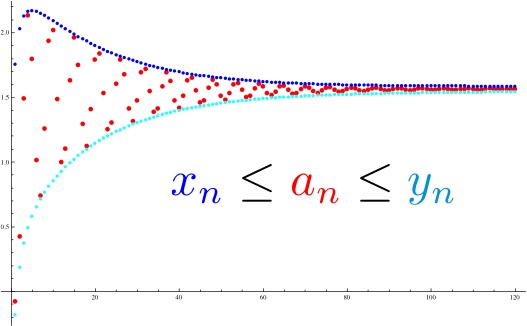
\includegraphics{./images/ch2/xay_n.jpg}}
\end{center}

{\bf 例:}证明$\limn [(n+1)^k-{n}^k]=0$,其中$0<k<1$。

[提示]:$n^k\left[\left(1+\df1n\right)^k-1\right]
<n^k\left(1+\df1n-1\right)=n^{k-1}\to 0\;(n\to\infty)$

\bigskip

{\bf 教材2.2.3节-例6:}{\b 设$a>0$为常数,证明$\limn \sqrt[n]{a}=1$。}
\ps{重点掌握结论!}

{\bf 例:}计算极限
\begin{enumerate}[(1)]
  \setlength{\itemindent}{1cm}
  \item $\limn\sqrt[n]{n^5}=1$
  \item $\limn\sqrt[n^2]{5^n+1}=1$
  \item 已知$a>b>0$,$\limn\sqrt[n]{\df1{a^n}+\df1{b^n}}=\df1b$
  \item 设$a_k\geq0,\;(k=1,2,\ldots)$,则$\limn\sqrt[n]
  {\sum\limits_{k=1}^na_k^n}=\max\limits_{1\leq k\leq n}a_k$
\end{enumerate}
 
{\bf 补充例题:}

{\bf 例:} $\limn\df{\sqrt{n+\sqrt n}-\sqrt n}{\sqrt[n]{3^n+5^n+7^n}}=\df1{14}$

% {\bf 例:} 已知$\limn a_n=A$,
% \begin{enumerate}[(1)]
%   \setlength{\itemindent}{1cm}
%   \item 证明:$\limn\df{[na_n]}n=A$
%   \item 若$\lambda\in(0,1)$,计算:
%   $$\limn(a_n+\lambda a_{n-1}+\lambda^2a_{n-2}+\ldots+\lambda^na_0)=\df
%   A{1-\lambda}$$
% \end{enumerate}

{\bf 例:} $\limn\sqrt[n]{n^5+5^n}=5$

{\bf 例:} 设$x\geq 0$,则
$\limn\sqrt[n]{1+x^n+\left(\df{x^2}2\right)^n}=
\left\{\begin{array}{ll}
1&x\in[0,1]\\ x & x\in(1,2]\\ \frac{x^2}2& x>2
\end{array}\right.$

{\bf 例:} $\limn\left(\df1{n+1}+\df1{\sqrt{n^2+1}}+\ldots
+\df1{\sqrt[n]{n^n+1}}\right)=1$

{\bf 例:}已知$k\in\mathbb{Z}_+$,计算:$\limn n^2\left(\df kn-\df1{n+1}-\df1{n+2}
-\ldots-\df1{n+k}\right)$

[提示]:
$$\df kn-\df1{n+1}-\df1{n+2}-\ldots-\df1{n+k}=\sum\limits_{i=1}^k\df{i}{n+i}$$
$$\df i{n(n+k)}\leq\df{i}{n+i}\leq\df i{n(n+1)}$$

\subsection{单调有界原理}

{\bf 定理2.2.5:}{\b 单调有界的数列必收敛。}\ps{只要数列从某一项开始单调即可!!!}

{\bf 证:}假设$\{a_n\}$单调递增有上界,由确界原理,可知其必有上确界,记为$A$。
以下证明$\limn a_n=A$。

事实上,对任意$\e>0$,由上确界的定义,必存在$a_N$,使得
$$A-\e<a_N\leq A.$$
由$\{a_n\}$单调递增,故对任意$n>N$,恒有$a_n\geq a_N$,又$a_n\leq A$,综上可知
$$|a_n-A|<\e,$$
由极限的定义,即证。


{\bf 【重要极限】}(教材2.2.4节-例7)\ps{重点掌握结论,证明了解即可}
$${\b a_n=\left(1+\df{1}{n}\right)^n\to e\quad (n\to\infty)}$$

[提示]:证明数列$\left\{\left(1+\df1n\right)^n\right\}$单调递增有上界。

先证有上界:

\begin{align}
	\left(1+\df1n\right)^n&=1+\df n1\cdot\df1n
	+\df{n\cdot(n-1)}{2\cdot1}\cdot\df1{n^2}+\ldots
	+\df{n\cdot(n-1)\ldots3\cdot2}{(n-1)\cdot(n-2)\ldots2\cdot1}\cdot\df1{n^2}\notag\\
	&<1+1+\df1{2\cdot1}+\ldots+\df1{(n-1)\cdot(n-2)\ldots2\cdot1}
	+\df1{n\cdot(n-1)\ldots2\cdot1}\notag\\
	&<1+1+\df12+\ldots+\df1{2^{n-2}}+\df1{2^{n-1}}<3\notag
\end{align}

再证单调性:

\begin{align}
	\left(1+\df1n\right)^n&=1+\df n1\cdot\df1n
	+\df{n\cdot(n-1)}{2\cdot1}\cdot\df1{n^2}+\ldots
	+\df{n\cdot(n-1)\ldots3\cdot2}{(n-1)\cdot(n-2)\ldots2\cdot1}
	\cdot\df1{n^{n-1}}\notag\\
	&\quad +\df{n\cdot(n-1)\ldots2\cdot1}{n\cdot(n-1)\ldots2\cdot1}
	\cdot\df1{n^{n}}\notag\\
	&=1+1+\df1{2\cdot 1}\left(1-\df1n\right)+\df1{3\cdot2\cdot
	1}\left(1-\df1n\right)\cdot\left(1-\df2n\right)+\ldots\notag\\
	&\quad +\df1{(n-1)\cdot(n-2)\ldots\cdot2\cdot
	1}\left(1-\df1n\right)\cdot\left(1-\df2n\right)
	\ldots\left(1-\df{n-2}n\right)\notag\\
	&\quad +\df1{n\cdot (n-1)\ldots\cdot2\cdot
	1}\left(1-\df1n\right)\cdot\left(1-\df2n\right)
	\ldots\left(1-\df{n-1}n\right)\notag\\
	&>1+1+\df1{2\cdot 1}\left(1-\df1{n-1}\right)+\df1{3\cdot2\cdot
	1}\left(1-\df1{n-1}\right)\cdot\left(1-\df2{n-1}\right)+\ldots\notag\\
	&\quad +\df1{(n-1)\cdot(n-2)\ldots\cdot2\cdot
	1}\left(1-\df1{n-1}\right)\cdot\left(1-\df2{n-1}\right)
	\ldots\left(1-\df{n-2}{n-1}\right)\notag\\
	&=\left(1+\df1{n-1}\right)^{n-1}\notag
\end{align}

{\bf 注:}需要掌握的重要性质{\b
\begin{itemize}
  \setlength{\itemindent}{1cm}
  \item 数列$\left\{\left(1+\df 1n\right)^n\right\}$严格单调递增有上界
  \item 数列$\left\{\left(1+\df 1n\right)^{n+1}\right\}$严格单调递减有下界
  \item 显然,二者极限相同
\end{itemize}}

{\bf 注意:}
{\b 典型错误
\begin{eqnarray*}
	\limn\left(1+\df1n\right)^n&
	=&\limn \underbrace{\left(1+\df 1n\right)\left(1+\df 1n\right)\cdots
	\left(1+\df	1n\right)}_{n}\\
	&=&\underbrace{\limn\left(1+\df1n\right)\limn\left(1+\df1n\right)
	\cdots\limn\left(1+\df1n\right)}_{n}\\
	&=&\left[\limn\left(1+\df1n\right)\right]^n=1
\end{eqnarray*}}
相当于$n$落在了极限符号之外,显然错误!!


\begin{shaded}
	{\bf 关于Napier常数$e$}
	
	{\bf 例:}若将$a>0$分成若干份,使得总乘积最大,由平均值不等式可知,显然
	等分最有利,但该分成多大的一份呢?分析可证明分成最接近于$e$的大小最合适。
	
	{\bf 例:}$\e_n=e-\sum\limits_{k=0}^n\df1{k!}$,则
	$$\limn\e_n(n+1)!=1$$
	
	[提示]:利用$\df00$型的Stolz定理
	
	{\bf 例:}$\delta_n=e-\left(1+\df1n\right)^n
	<\left(1+\df1n\right)^{n+1}-\left(1+\df1n\right)^n
	=\left(1+\df1n\right)^n\df1n<\df en<\df3n$
	
	事实上,$\limn\df{2n\delta_n}e=1$
	
	{\bf 重要不等式:}由{$\left(1+\df1n\right)^n<e<\left(1+\df1n\right)^{n+1}$},
	可得
	$${\b \df1{n+1}<\ln\left(1+\df1n\right)<\df1n}$$

	{\bf 例:}证明$a_n=\df1{n+1}+\ldots+\df1{2n},\;(n\in\mathbb{Z}_+)$收敛。

	[提示]:利用$\df1{n+1}<\ln\left(1+\df1n\right)<\df1n$,极限为$\ln2$
% 	
% 	{\bf Eular常数:}
% 	$$\gamma=\limn\left(\sumn\df1k-\ln n\right)\approx 0.5772\ldots$$
\end{shaded}

\subsection{递推数列的判敛}

{\bf 例:}已知$a_1,a_2$为常数,数列$\{a_n\}$满足:
$$a_n=\df 12({a_{n-1}+a_{n-2}})\quad(n>2).$$
证明$\{a_n\}$收敛,并求其极限。\ps{\b 熟练掌握此类递推!!!}

{\bf 解:}原递推式可改写为
$$a_n-a_{n-1}=-\df12(a_{n-1}-a_{n-2})\quad(n>2),$$
由此递推,易得
$$a_n-a_{n-1}=\left(-\df12\right)^{n-2}(a_2-a_1),$$
进而
\begin{align}
	a_n&=a_{n-1}+\left(-\df12\right)^{n-2}(a_2-a_1)\notag\\
	&=a_{n-2}+\left[\left(-\df12\right)^{n-3}+\left(-\df12\right)^{n-2}\right]
	(a_2-a_1)\notag\\
	&=\ldots\notag\\
	&=a_2+\left[\left(-\df12\right)+\ldots+\left(-\df12\right)^{n-3}
	+\left(-\df12\right)^{n-2}\right](a_2-a_1)\notag\\
	&=a_2-\df12\df{1-\left(-\df12\right)^{n-2}}{1+\df12}(a_2-a_1)\notag\\
	&\to\df13a_1+\df23a_2\;(n\to\infty)\notag
\end{align}
即证。

\begin{shaded}
	{\bf 特征根法求解求解二阶常系数齐次递推}
	
	{\bf 注:}中学阶段,有些同学接触过所谓的特征根法求递推公式,具体过程如下,其背后
	的原理与上面一个例子中的方法是完全一致的。
	
	已知$a_1,a_2$和如下的递推式:
	
	$$a_{n+2}=Aa_{n+1}+Ba_n\quad (AB\ne 0, A+B\ne 1),$$
	求$\{a_n\}$的通项公式。
	
	考虑特征方程:
	$$r^2=Ar+B$$
	\begin{enumerate}[(1)]
	  \setlength{\itemindent}{1cm}
	  \item 若特征方程有相异实根$p,q$,则
	  $$a_n=C_1p^n+C_2q^n$$
	  其中系数$C_1,C_2$由方程
	  $$\left\{\begin{array}{l}
	  a_1=C_1p+C_2q\\
	  a_2=C_1p^2+C_2q^2
	  \end{array}\right.$$
	  可解得
	  $$C_1=\df{a_1q-a_2}{p(q-p)},\quad 
	  C_2=\df{a_1p-a_2}{q(p-q)}$$
	  \item 若有两个相等的实根$r$,则
	  $$a_n=[C_1r+C_2(n-1)]r^{n-1}$$
	  与(1)类似地可求出系数$C_1,C_2$
	\end{enumerate}
	
	{\bf 例:}Fibonacci数列:$a_{n+2}=a_n+a_{n+1},\;a_1=a_2=1$
	
	$$a_n=\df1{\sqrt5}\left[\left(\df{1+\sqrt5}2\right)^n
	-\left(\df{1-\sqrt5}2\right)^n\right]$$
	
\end{shaded}

{\bf 教材2.2.5节-例9:}设$a_1>0$,$a_{n+1}=\df 12\left(a_n+\df 1{a_n}\right)\,
(n=1,2,\ldots)$,证明$\{a_n\}$收敛,并求其极限。

解答略。

{\bf 小结:}求解递推数列的极限问题,注意以下几点:{\b
\begin{itemize}
  \setlength{\itemindent}{1cm}
  \item 递推式两边同时取极限,解方程求得极限的值,是最便利的计算递推数列极限的方法
  \item 若通过以上方法可以求出极限的值,通常只需证明数列单调有界即可
  \item 若该方法无法求得极限的值,则只能利用递推式推导数列通项,进而证明其收敛并计算极限
\end{itemize}}

{\bf 例:}证明极限存在,然后求出极限的值
\begin{enumerate}[(1)]
  \setlength{\itemindent}{1cm}
  \item $\limn\df{n^2}{a^n}\quad (a>1)$%\hfill({\it 单调递减有下界,极限为$0$})
  \ps{\b 由(1)可推广得到一个常用的结论:$b>0,|a|<1$,则$n^ba^n\to 0$}
  \item $\limn\df{n!}{n^n}$%\hfill({\it 单调递减有下界,极限为$0$})
%   \item 设$c>0$,求$\limn\underbrace{\sqrt{c
%   +\sqrt{c+\ldots+\sqrt{c}}}}_{n\mbox{\small 个根号}}$
\end{enumerate}

{\bf 解:}(1)\;记$b_n=\df{n^2}{a^n}$,则
$$b_{n+1}=\df{(n+1)^2}{n^2a}b_n,$$
注意到$\limn\df{b_{n+1}}{b_n}=\df1a<1$,故当$n$充分大时,$\{b_n\}$严格单调递减,
而显然$b_n>0$,故由单调有界原理,$\{b_n\}$收敛,设其极限为$A$。在前述递推式两端同时取极限,
可得
$$A=\df1aA\quad\Rightarrow\quad A=0,$$
即为所求。

(2)\;类似解法,略。

{\bf 注:}{\b 若极限存在,可由通项公式反推递推式,然后两边取极限,解方程求得极限值}

{\bf 补充例题:}

{\bf 例:}$x_1=\df c2$,$x_{n+1}=\df c2+\df{x_n^2}2\,(n\in\mathbb{Z}_+)$,
证明:若$c>1$,则$\{x_n\}$发散。

[提示]:设极限为$A$,则$A^2-2A+c=0$,$c>1$时,无解,必发散。

{\bf 例:}$a_0>b_0>0$,
$$a_n=\df12(a_{n-1}+b_{n-1}),\quad
b_n=\sqrt{a_{n-1}b_{n-1}}\;(n\in\mathbb{Z}_+)$$
证明:$\{a_n\},\{b_n\}$收敛于同一极限。

[提示]:$b_0<b_1<a_1<a_0$,利用数学归纳法证明:
$$b_0<b_1<\ldots<b_n<a_n<\ldots<a_1<a_0$$

{\bf 例:}证明:$a_n=\sqrt{1+\sqrt{2+\ldots+\sqrt{n}}}$收敛。

[提示]:注意到
$$\sqrt{n-1+\sqrt n}<\sqrt{n-1+2\sqrt{n-1}+1}=\sqrt{n-1}+1,$$
然后利用不等式$\sqrt{n-1}<2\sqrt{n-2}$递推。

{\bf 例:}给定$x\in(0,3),\; x_{n+1}=\sqrt{x_n(3-x_n)},\;(n\in\mathbb{Z}_+)$,
证明数列$\{x_n\}$收敛,并求其极限。

[提示]:$0<x_2\leq\df12[x_1+(3-x_1)]=\df32$,递推可得
$0<x_n\leq\df32$。另一方面,
$$x_{n+1}-x_n=\df{\sqrt{x_n}(3-2x_n)}{\sqrt{x_n(3-x_n)}+\sqrt{x_n}}\geq 0.$$
即$\{x_n\}$单调递增有上界。

{\bf 例:}证明数列$\{x_n\}:x_1=1,\;x_{n+1}=\df1{1+x_n}$收敛,求其极限。

[提示]:由递推式易得极限$a=\df{\sqrt5-1}2$。(写成:$a$为满足方程$a=\df1{1+a}$的正数)

显然$0<x_n\leq1$,进而$\df1{1+x_n}\geq\df12$。于是\ps{$\{x_n\}$不单调!}
\begin{align}
	|x_{n+1}-a|&=\left|\df1{1+x_n}-\df1{1+a}\right|=\df{|x_n-a|}{(1+x_n)(1+a)}\notag\\
	&<\df{|x_n-a|}{(1+1/2)(1+1/2)}=\df49|x_n-a|\notag\\
	&<\left(\df49\right)^2|x_{n-1}-a|<\ldots<\left(\df49\right)^{n}|x_1-a|,\notag
\end{align}
由夹逼定理可知$|x_{n+1}-a|\to0\;(n\to\infty)$,即证。

\subsection{Stolz定理}

{\b{\bf Stolz定理}
\ps{Stolz定理类似于函数极限中的L'Hospital法则,例如:
对比$\limn\df{n^2}{e^n}$和$\limx{+\infty}\df{x^2}{e^x}$}
($\df{\infty}{\infty}$形式) 设数列$\{y_n\}$满足$\limn\df
1{y_n}=0$,且$\{y_n\}$至少从某一项开始保持严格单调递增,
则对任意数列$\{x_n\}$,若$\limn\df{x_n-x_{n-1}}{y_n-y_{n-1}}$存在,则必有
$$\limn\df{x_n}{y_n}=\limn\df{x_n-x_{n-1}}{y_n-y_{n-1}}$$

% {\bf 注:}Stolz定理主要用于计算"$\df{\infty}{\infty}$型"的极限

{\bf 推论}(Cauchy极限定理)若$\{a_n\}$收敛,则
$$\limn\df{a_1+a_2+\ldots+a_n}n=\limn a_n$$}

{\bf 例:}计算以下极限
\begin{enumerate}[(1)]
  \setlength{\itemindent}{1cm}
  \item $\limn\df{1+\sqrt 2+\sqrt[3]{3}+\ldots+\sqrt[n]{n}}{n}$ 
  \item $\limn\df{1^k+2^k+\ldots+n^k}{n^{k+1}},\quad(k\in\mathbb{N})$ 
  \item $\limn\left(\df{1^k+2^k+\ldots+n^k}{n^{k}}-\df
  n{k+1}\right),\quad(k\in\mathbb{N})$
\end{enumerate}
  
  [提示]:(3)以下$P^{(*)}_k(n)$表示以$n$为变量的$k$次多项式,
  \begin{eqnarray*}
  	\mbox{原式}&=&\limn\df{(k+1)(1^k+2^k+\cdots+n^k)-n^{k+1}}{n^k(k+1)}\\
  	&=&\limn\df{(k+1)(n+1)^k-[(n+1)^{k+1}-n^{k+1}]}{(k+1)[(n+1)^k-n^k]}\\
  	&=&\limn\df{(k+1)[n^k+kn^{k-1}+P_{k-2}^{(1)}(n)]
  	-\left[(n+1)^k+(n+1)^{k-1}n+\cdots+n^k\right]}{(k+1)
  	\left[(n+1)^{k-1}+(n+1)^{k-2}n+\cdots+n^{k-1}\right]}\\
  	&=&\limn\df{(k+1)[n^k+kn^{k-1}+P_{k-2}^{(1)}(n)]-(k+1)n^k
  	-\df{k(k+1)}2n^{k-1}-P_{k-2}^{(2)}(n)}
  	{(k+1)\left[\df{k(k+1)}{2}n^{k-1}+P_{k-2}^{(3)}(n)\right]}\\
  	&=&\df12
  \end{eqnarray*}


{\b{\bf 推论:}设$\{a_n\}$为正数列,则
$$\limn\sqrt[n]{a_1a_2\ldots a_n}=\limn a_n$$

{\bf 推论:}设$\{a_n\}$为正数列,$\limn\df{a_{n+1}}{a_n}=q$,
则$\limn\sqrt[n]{a_n}=q$}

[提示]:设$b_1=a_1,\;b_n=\df{a_n}{a_{n-1}}$,利用上一推论即可。

{\bf 例:}计算极限$\limn\df{\sqrt[n]{n!}}{n}$

[提示]:记$b_n=\df{n!}{n^n}$,由以上推论
$$\limn\sqrt[n]{b_n}=\limn\df{b_{n+1}}{b_n}=\df1e$$

{\bf 例:}计算$\limn\df{1!+2!+\ldots+n!}{n!}=1$

{\b{\bf Stolz定理}($\df00$型)设$\limn a_n=\limn b_n=0$,且$\{a_n\}$严格
单调递减,若$\limn\df{b_{n+1}-b_n}{a_{n+1}-a_n}=l$($l$可以为$\pm\infty$),
则$\limn\df{b_n}{a_n}=l$}

[提示]:证明中用到如下不等式:若$\df{p_i}{q_i}\in(a,b)\;(q_i>0,i=1,2,\ldots,n,)$
则
$$\df{\sum\limits_{i=1}^np_i}{\sum\limits_{i=1}^nq_i}\in(a,b)$$

{\bf 补充例题:}

% {\bf 例:}设$\limn a_n=\alpha,\limn b_n=\beta$,则
% $$\limn\df{a_1b_n+a_2b_{n-1}+\ldots+a_nb_1}n=\alpha\beta$$

{\bf 例:}$\limn\df{\ln n}{1+\frac12+\ldots+\frac1n}=1$

{\bf 例:} 设$\limn a_n=a$,证明:
\begin{enumerate}[(1)]
  \setlength{\itemindent}{1cm}
  \item $\limn\df{a_0+a_1+\ldots+na_n}{n^2}=\df a2$
  \item $\limn\df{a_1+\frac12a_2+\ldots\frac1na_n}{\ln n}=a$
\end{enumerate}

{\bf 例:}若$\limn x_n=a$,极限$\limn\df{x_{n+1}}{x_n}$是否一定存在

{\bf 答:}不一定。反例:$x_n=\df1{3^{[\frac{n+1}2]}}$ (也即
$\df13, \df13, \df 1{3^2}, \df1{3^2}, \df1{3^3}, \df1{3^3},\ldots$)

{\bf 讨论:}若$\limn x_n=a\ne 0$,则极限$\limn\df{x_{n+1}}{x_n}$一定存在!
为什么$a=0$时的结论就为不一定呢?\ps{因为此时极限为$\df00$型的不定式极限}

\newpage

\section{数值级数}

\subsection{无穷和的定义}

{\bf 级数(无穷和):}无穷多个数按照一定{\it 次序}求和
\ps{更严谨的说法应该是:\b 对给定的数列按照顺序求和(所形成的部分和数列)}
$$\sum\limits_{k=1}^{\infty}a_k
=\lim_{n\to\infty}\left(\sum_{k=1}^na_k\right)$$  
其中$a_k\in\mathbb{R}\,(k\in\mathbb{N})$。
\ps{正确理解级数的定义是理解其各种性质的关键}

\begin{itemize}
  \item {\bf 部分和(数列):}
  $$S_n=\sum\limits_{k=1}^na_k$$
  \item {\bf 级数收敛}$\Leftrightarrow\{S_n\}$收敛
\end{itemize}

{\bf 例:}判断下列级数的收敛性
\begin{enumerate}[(1)]
  \setlength{\itemindent}{1cm}
  \item $\sumn q^n\quad (q>0)$ \quad({\it\b 几何级数,$|q|<1$时收敛}) 
  \item $\sumn\df{1}{n(n+1)}=1$\quad\ps{“裂项”——有理函数分解}
  \item $\sumn\df 1n$ \quad({\it\b 调和级数,发散})\\ 
  提示:$$S_{2n}-S_n=\df1{2n}+\df1{2n-1}+\ldots+\df1n
  >n\cdot\df1{2n}=\df12$$
  由此进而易知$\{S_n\}$无界,从而发散!
% 		  \item $\sumn\df 1n^2$
  \item $\sumn (-1)^n$ \quad({\it 发散})
\end{enumerate}

\begin{shaded}

% \begin{figure}[!htp]
% 	\centering
% 	\begin{minipage}[b]{0.2\textwidth}
% 		\resizebox{!}{4cm}{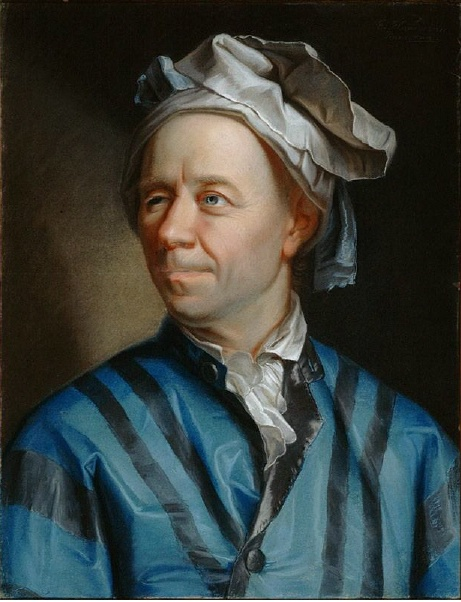
\includegraphics{./images/ch2/Euler.jpg}}
% 	\end{minipage}\quad
% 	\begin{minipage}[b]{0.7\textwidth}
% 		{\bf 【关于调和级数】}
% 		
% 		调和级数发散的速度慢得让人有些不可思议,其前$1000$项的和约为$7.485$,
% 		前$100$万项的和约为$14.357$,前$10$亿项的和约为$21$,前一万亿项和约为$28$,
% 		当它的和超过$100$时,如果每一项在纸带上只占$1$毫米,我们必须使用$10^{43}$毫米长
% 		的纸带,这大约是$10^{25}$光年,而宇宙估计尺寸只有$10^{12}$光年,
% 		因此也难怪大家都会认为它是收敛的。
% 	\end{minipage}
% \end{figure}
% \begin{wrapfigure}{r}{2cm}
% 	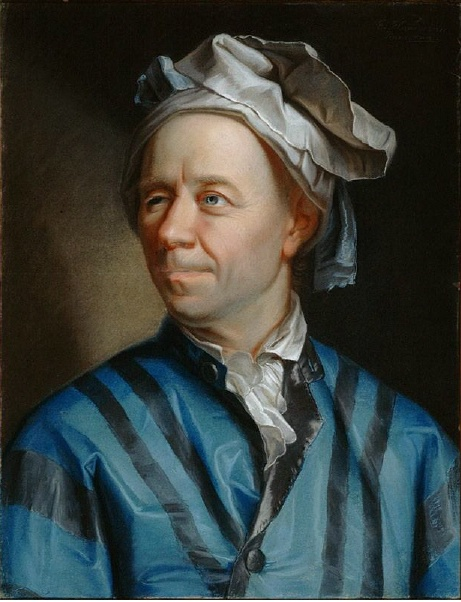
\includegraphics{./images/ch2/Euler.jpg}
% % 	\caption{Leonhard Euler\,(1707-1783)}
% % 	\label{fig:Euler}
% \end{wrapfigure}

% \begin{tabular}{p{0.2\textwidth}p{0.7\textwidth}}
% 	\resizebox{!}{4cm}{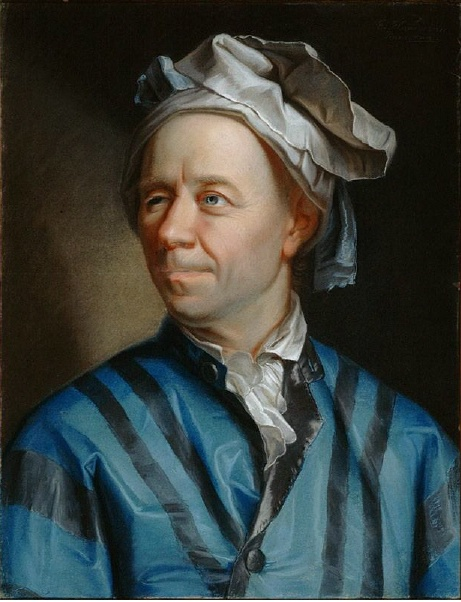
\includegraphics{./images/ch2/Euler.jpg}}
% 	&
% 	{\bf 【关于调和级数】}
% 	
% 	调和级数发散的速度慢得让人有些不可思议,其前$1000$项的和约为$7.485$,
% 	前$100$万项的和约为$14.357$,前$10$亿项的和约为$21$,前一万亿项和约为$28$,
% 	当它的和超过$100$时,如果每一项在纸带上只占$1$毫米,我们必须使用$10^{43}$毫米长
% 	的纸带,这大约是$10^{25}$光年,而宇宙估计尺寸只有$10^{12}$光年,
% 	因此也难怪大家都会认为它是收敛的。
% \end{tabular}

{\bf 【关于调和级数】}

调和级数发散的速度慢得让人有些不可思议,其前$1000$项的和约为$7.485$,
前$100$万项的和约为$14.357$,前$10$亿项的和约为$21$,前一万亿项和约为$28$,
当它的和超过$100$时,如果每一项在纸带上只占$1$毫米,我们必须使用$10^{43}$毫米长
的纸带,这大约是$10^{25}$光年,而宇宙估计尺寸只有$10^{12}$光年,
因此也难怪大家都会认为它是收敛的。

% \begin{center}
% 	\resizebox{!}{4cm}{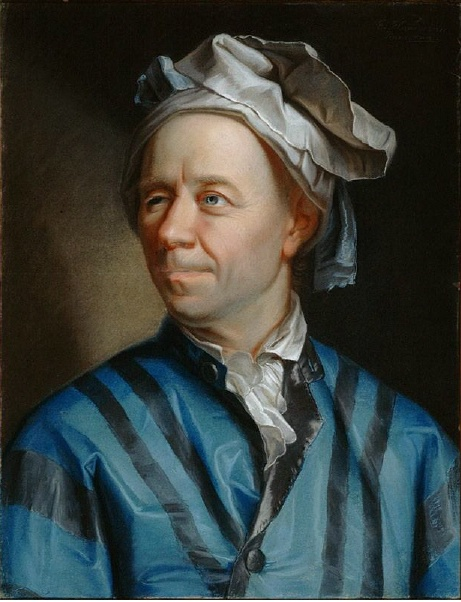
\includegraphics{./images/ch2/Euler.jpg}}
% \end{center}

{\bf 【Euler常数】}

Euler常数最先由瑞士数学家莱昂哈德·欧拉(Leonhard Euler)
在1735年发表的文章 De Progressionibus harmonicus observationes 中定义。
欧拉曾经使用C作为它的符号,并计算出了它的前6位小数。1761年他又将该值计算到了16位小数。
$$\gamma=\limn\left[\sum\limits_{k=1}^n\df1k-\ln n\right]
=\int_1^{\infty}\left(\df1{[x]}-\df1x\right)\d x$$
由不等式$\ln(1+x)<x,(x\in(-1,+\infty),x\ne 0)$,
$$S_n=\sum\limits_{k=1}^n\df1k-\ln n>\sum\limits_{k=1}^n
\ln\left(1+\df1k\right)-\ln n=\ln(n+1)-\ln n>0.$$
$$S_n-S_{n+1}=\ln(n+1)-\ln n-\df1{n+1}>-\left(-\df1{n+1}\right)
-\df1{n+1}=0.$$
由单调有界原理可知$\{S_n\}$收敛。
\end{shaded}

\subsection{收敛级数的性质}

\begin{enumerate}[{\bf 【性质1】}]
  \item {\bf 定理2.3.1}(级数收敛的必要条件) 
  $$\sumn a_n\mbox{收敛}\Rightarrow\limn a_n=0$$
  
  {常用于判定级数发散:\b 若$\{a_n\}$不以$0$为极限,则$\sumn a_n$发散}
  \item {\b$\sumn
  a_n$收敛$\Leftrightarrow\sum\limits_{n=k}^{\infty}a_n$收敛$(k\in\mathbb{N})$}\\
  (因此,讨论收敛性时只需考虑“最后部分”的部分和)
  \ps{类似于数列的收敛性只与其“尾部”的数字有关}
  \item {\bf 教材2.3.1节-例2:}$\{a_n\}$收敛$\Leftrightarrow\sumn(a_{n+1}-a_n)$收敛
  \item {\bf 定理2.3.2-3:}两个收敛级数的线性组合仍然收敛
  \ps{类似于收敛数列的线性组合仍收敛}  
  \item {\bf 定理2.3.4:}{\b 增加、减少或改变级数中的有限项不影响其敛散性} 
  \ps{与性质2类似,增减或改变数列中的有限项不改变其敛散性}
  \item {\bf 定理2.3.5:}若$\sumn a_n$收敛,不改变求和顺序,
  任意合并其中的项,所得新的级数仍收敛 
  \begin{itemize}
    \item {\bf 推论:}合并收敛级数中的相邻项,所得级数仍收敛 
    \ps{\b 合并相邻项相当于取$\{S_n\}$的偶子列$\{S_{2n}\}$}
    \item {{对发散级数,该性质不成立}} 
    {例:$\sumn(-1)^n$}
    \item {{\b 改变求和次序,可能改变级数的收敛和}},例:$\sumn\df{(-1)^n}n$
  \end{itemize}
%   \item (Cauchy原理)级数$\sumn a_n$收敛当且仅当:$\forall\e$,
%   $\exists N\in\mathbb{Z}$,使对$\forall n>N$和$\forall p\in\mathbb{Z}^+$,
%   都有
%   $$|a_{n+1}+a_{n+2}+\ldots+a_{n+p}|<\e.$$
\end{enumerate}

% {\bf 例:}判断以下级数的敛散性;若收敛,求其和
% 
% \begin{enumerate}[(1)]
%   \setlength{\itemindent}{1cm}
%   \item $\sumn\ln\left(1+\df 1n\right)$
%   \item
%   $\sumn\left[\prod\limits_{k=0}^p(\alpha+n+k)\right]^{-1},\;(p\in\mathbb{N})$
%   \item $\sumn\df{x^{2^{n-1}}}{1-x^{2n}}$
%   \item $\sumn\df{1}{\sqrt n}$
% \end{enumerate}

% {\bf 例:}利用Cauchy原理证明$\sumn\df1{n^2}$收敛
% 
% \begin{align}
% 	&|a_{n+1}+a_{n+2}+\ldots+a_{n+p}|\notag\\
% 	&<\df1{(n+1)(n+2)}+\df1{(n+2)(n+3)}+\ldots+\df1{(n+p-1)(n+p)}\notag\\
% 	&=\df1n-\df1{n+p}<\df1n\notag
% \end{align}

{\bf 注:}直接使用比较判别法证明更为简洁

{\bf 例:}判断正误:
\begin{enumerate}[(1)]
  \setlength{\itemindent}{1cm}
  \item $\{a_n\}$与$\sumn a_n$同敛散\hfill$\times$
  \item $k\ne 0$则$\sumn a_n$与$\sumn ka_n$同敛散\hfill$\surd$
  \item $\sumn a_n$收敛,$\sumn b_n$发散,则$\sumn(a_n+b_n)$发散\hfill$\surd$
  \item $\sumn a_n$与$\sumn b_n$均发散,则$\sumn(a_n+b_n)$发散\hfill$\times$
  \item 若$\sum\limits_{n=1}^{\infty}a_{2n}$和
  $\sum\limits_{n=1}^{\infty}a_{2n-1}$均收敛,则$\sumn a_n$收敛\hfill$\surd$
  \item 若$\sum\limits_{n=1}^{\infty}(a_{2n}+a_{2n-1})$收敛,则
  $\sumn a_n$收敛\hfill$\times$
\end{enumerate}

{\bf 例:} 求和$\sumn\df1{n(n+1)(n+2)}=\df14$

{\bf 例:}求和 $\sumn\df{n}{3^n}$

[提示]:记$S_n=\df13+\df2{3^2}+\ldots+\df n{3^n}$,则
$$\df13S_n=\left(\df1{3^2}+\df2{3^3}+\ldots
+\df{n-1}{3^n}\right)+\df{n}{3^{n+1}}$$
因此
$$\df23S_n=\df12\left(1-\df1{3^n}\right)-\df{n}{3^{n+1}}\to\df12
(n\to\infty)$$

\section{同号级数的收敛性}

\subsection{同号级数收敛的充要条件}

{\bf 定理2.4.1:}正项级数收敛,当且仅当其部分和数列有界。\ps{相当于数列收敛的单调有界原理}

{\bf 教材2.4.1-例1:}证明$\sumn\df1{n!}$收敛。

解答略。

\subsection{比较判别法}

{\bf 定理2.4.2}(比较判别法的不等式形式)若对充分大的$n$,总有$0\leq a_n\leq b_n$,则
% \ps{相当于数列收敛的夹逼定理}
\begin{enumerate}
  \setlength{\itemindent}{1cm}
  \item 若$\sumn b_n$收敛,则$\sumn a_n$收敛
  \item 若$\sumn a_n$发散,则$\sumn b_n$发散
\end{enumerate}

{\bf 注:}{\b 对于变号(非同号)级数,比较判别法不成立},例:
$$a_n=-\df1n+\df{(-1)^n}{\sqrt n}<\df{(-1)^n}{\sqrt n}=b_n,$$
可以证明$\sumn b_n$收敛,但$\sumn a_n$发散。

{\bf P66-例3:}证明:$p$-级数\ps{$p$-级数常常用作与其他级数比较判敛的“标杆”}
\begin{enumerate}[(1)]
  \setlength{\itemindent}{1cm}
  \item[(1)] $p>1$时,$\sumn\df1{n^p}$收敛;
  \item[(2)] $0<p\leq 1$时,$\sumn\df1{n^p}$发散。
\end{enumerate}

[提示]:(2),$p=1$时,显然发散。又因为
$$0<\df 1n<\df 1{n^p},\quad (0<p<1),$$
已知调和级数发散,故$p$-级数发散;

\begin{shaded}
(1)由以下推导可知$p>1$时,$p$-级数的部分和数列有界
\begin{eqnarray*}
	S_{(2^k)^p}&=&1+\df 1{2^p}+\underbrace{\left(\df1{3^p}+\df1{(2^2)^p}\right)}_2
				+\underbrace{\left(\df1{5^p}+\ldots+\df1{(2^3)^p}\right)}_{2^2}+\ldots\\
				&&+\underbrace{\left[\df1{(2^{k-1}+1)^p}+\ldots+\df1{(2^k)^p}\right]}_{2^{k-1}}\\
			  &\leq &1+\df 1{2^p}+2\cdot\df1{2^p}+2^2\cdot\df1{(2^2)^p}
			    +\ldots+2^{k-1}\cdot\df1{(2^{k-1})^p}\\
			  &=&1+\df 1{2^p}+\left[\df1{2^{p-1}}+\left(\df1{2^{p-1}}\right)^2+
			    \ldots+\left(\df1{2^{p-1}}\right)^{k-1}\right]\\
			  &=&1+\df 1{2^p}+\df1{2^{p-1}}\df{1-\left(\df1{2^{p-1}}\right)
			    ^{k-1}}{1-\df1{2^{p-1}}}<1+\df 1{2^p}+\df1{2^{p-1}-1}
\end{eqnarray*}
\end{shaded}


{\bf 例:}讨论下列级数的敛散性
\begin{enumerate}[(1)]
  \setlength{\itemindent}{1cm}
  \item[(1)] $\sumn\df{1}{3^{\ln n}}$
  \hfill({[提示]:$a^{\ln b}=b^{\ln a},\;(a,b>0)$})
  \item[(2)] $\sum\limits_{n=2}^{\infty}\df 1{(\ln n)^{\ln n}}$
  \item[(3)] $\sum\limits_{n=3}^{\infty}\df 1{(\ln n)^{\ln\ln n}}$
\end{enumerate}
	
[提示]: (2)\;当$n>e^{e^2}$时,
$$(\ln n)^{\ln n}=n^{\ln\ln n}>n^2.$$

(3)\;注意到$n$充分大时,$\ln n<\sqrt{n}$,进而$(\ln\ln n)^2<\ln n$,故有
  $$\df 1{(\ln n)^{\ln\ln n}}=\df 1{e^{(\ln\ln
  n)^2}}>\df 1n$$

\begin{shaded}
	{\bf 一点“常识”}
	
	{\b 设$\e>0, a>1$,则对于充分大的$n$,总成立如下关系
	$$\ln n<<n^{\e}<<a^n<<n!<<n^n$$}

	学习了函数极限的L'Hospital法则后,能够比较容易地验证以上结论。
	
	{\bf 例:} 对于充分大的$x$,$e^x>2x^4$,故对充分大的$n$,
	有$e^{\sqrt[3]n}>2n^{\frac 43}$,从而可知$\sumn e^{-\sqrt[3]n}$收敛
\end{shaded}

{\bf 教材2.4.2节-例4:}设$a_n\leq c_n\leq b_n\;(n\in\mathbb{N})$,$\sumn a_n,\sumn
b_n$均收敛, 则$\sumn c_n$收敛。
\begin{itemize}
  \setlength{\itemindent}{1cm}
  \item 类似于数列收敛的“夹逼定理”
  \item {\b 该结论不要求必须是正项级数}
\end{itemize}

{\bf 推论}(定理2.5.2)若级数$\sumn|a_n|$收敛,则$\sumn a_n$也收敛。

[提示]:
$$-|a_n|\leq a_n\leq|a_n|$$

{\bf 定理2.4.3}(比较判别法的极限形式)已知$a_n,b_n$均非负$(n\in\mathbb{Z}_+)$,
且$\limn\df{a_n}{b_n}=l$,则 
\begin{enumerate}
  \setlength{\itemindent}{1cm}
  \item 若$0<l<+\infty$,$\sumn a_n,\sumn b_n$同敛散 \hfill({\it 随着$n$的增大,
  $a_n,b_n$的比值趋于常数})
  \item 若$l=0$,$\sumn b_n$收敛$\Rightarrow\sumn a_n$收敛 
  \hfill({\it 随着$n$的增大,$a_n$的值远小于$b_n$})
  \item 若$l=+\infty$,$\sumn a_n$收敛$\Rightarrow\sumn b_n$收敛
  \hfill({\it 随着$n$的增大,$a_n$的值远大于$b_n$})
\end{enumerate}

{\bf 教材2.4.2节-例5-6:}判断以下级数的收敛性
\begin{enumerate}[(1)]
  \setlength{\itemindent}{1cm}
  \item $\sumn\df 1{2^n}\df{n^2+1}{2n^2-1}$ 
  \item $\sumn\df{n+1}{n^k+2}\quad (k=1,2,\ldots)$ 
  \item $\sumn\df{1}{n\sqrt[n]{n}}$ 
  \item $\sumn\df{1}{1+x^n}\quad(x>0)$
\end{enumerate}

{\bf 推论}($p$-判别法)设$a_n\geq 0\;(n=1,2,\ldots)$,则\ps{指定$p$-级数作为比较的对象} 
\begin{enumerate}
  \setlength{\itemindent}{1cm}
  \item 若存在$p>1$,使得$\limn n^pa_n$存在,则$\sumn a_n$收敛 
  \item 若$0<p\leq 1$,使得$\limn n^pa_n>0$,则$\sumn a_n$发散
\end{enumerate}

{\bf 例:}判断以下级数的收敛性
\begin{enumerate}[(1)]
  \setlength{\itemindent}{1cm}
  \item $\sumn\df{\arctan n}{n^{3/2}}$
  \item $\sumn\df{\ln n}{n^{5/4}}$\ps{任何正幂次函数的增长速度最终都比任意对数函数快}
\end{enumerate}

{\bf 例:}$\sumn a_n$、$\sumn b_n$均为正项级数,若对充分大的$n$,总有
$$\df{a_{n+1}}{a_n}\leq\df{b_{n+1}}{b_n},$$
则若$\sumn b_n$收敛,$\sumn a_n$收敛。

[提示]:
$$a_{n+1}\leq\df{a_1}{b_1}b_{n+1}$$

{\bf 补充例题:}

{\bf 例:}(2012年全国大学生数学竞赛)
$\sumn a_n$和$\sumn b_n$均为正项级数,证明:
\begin{enumerate}
  \setlength{\itemindent}{1cm}
  \item 若$\limn\left(\df{a_n}{a_{n+1}b_n}-\df 1{b_{n+1}}\right)>0$,
  则$\sumn a_n$收敛;
  \item 若$\limn\left(\df{a_n}{a_{n+1}b_n}-\df 1{b_{n+1}}\right)<0$,
  且$\sumn b_n$发散,则$\sumn a_n$发散。
\end{enumerate}

[提示]:1. 由已知,存在$q>0$和$N\in\mathbb{Z}_+$,对任意$n\geq N$,有
$$\df{a_n}{a_{n+1}b_n}-\df 1{b_{n+1}}>q,$$
从而
$$a_{n+1}<\df1q\left(\df{a_n}{b_n}-\df{a_{n+1}}{b_{n+1}}\right).$$
利用递推关系可得
$$\sum\limits_{k=N}^na_k<a_N+\df1q\left(\df{a_N}{b_N}-\df{a_n}{b_n}\right)
<a_N+\df1q\df{a_N}{b_N},$$
故$\sumn a_n$部分和有界,从而收敛。

2.$n$充分大($n>N$)时,有
$$a_{n+1}>\df{b_{n+1}}{b_n}a_n>\ldots>
\df{b_{n+1}}{b_n}\df{b_{n}}{b_{n-1}}\ldots\df{b_{N+1}}{b_N}a_N
=\df{a_N}{b_N}b_{n+1},$$
由比较判别法,$\sumn b_n$发散,则$\sumn a_n$发散。

{\bf 例:} $\sumn\left(\cot\df{n\pi}{4n-2}-\sin\df{n\pi}{2n+1}\right)$

[提示]:考虑$\sumn\left(1-\cot\df{n\pi}{4n-2}\right)$和
$\sumn\left(1-\sin\df{n\pi}{2n+1}\right)$,注意到
$$\limn\df{1-\sin\df{n\pi}{2n+1}}{\df1n}=\df{\pi}4,
\quad\limn\df{1-\sin\df{n\pi}{2n+1}}{\df1{n^2}}=\df{\pi^2}{32},$$
故以上级数一个发散一个收敛,从而原级数发散。

{\b\bf 牢记:比较判别法仅对同号级数有效!!!}

\subsection{比值判别法}

{\bf 定理2.4.4}(d'Alembert判别法)
设$a_n\geq 0(n=1,2,\ldots)$,$\limn\df{a_{n+1}}{a_n}=q$,则
\ps{极限形式,掌握结论,不要求会证明} 
\begin{enumerate}
  \setlength{\itemindent}{1cm}
  \item $0\leq q<1\Rightarrow\sumn a_n$收敛 
  \item $q>1\Rightarrow\sumn a_n$发散
\end{enumerate}

{\bf 注:}$q=1$时,比值判别法无法给出确定的结论,例如:$\sumn\df 1n$
和$\sumn\df 1{n^2}$都对应于$q=1$,但前者发散,后者收敛

{\bf 教材2.4.3节-例5-7:}判断下列级数的收敛性
\begin{enumerate} [(1)]
  \setlength{\itemindent}{1cm}
  \item $\sumn\df 1{2^n}\df{n^2+1}{2n^2-1}$ 
  \item $\sumn\df{n^2}{2^n}$ 
  \item $\sumn\df{(2n)!}{(n!)^2}$
%   \item $\sumn n!\left(\df{x}{n}\right)^n\quad (x>0)$
\end{enumerate}

{\bf 例:}设$t>0$,讨论级数$\sumn\df{t^nn!}{n^n}$的敛散性。

[提示]:若$t=e$,
$$\df{a_{n+1}}{a_n}=\df{e}{\left(1+\df1n\right)^n}>1,$$
故$\{a_n\}$必不以$0$为极限,可知$\sumn a_n$发散;

$t\ne e$的情况利用比值判别法即可判断。

{\bf 注:}考虑$\sumn\df{n^n}{e^nn!}$,
则以上推导不再成立,该如何判定其敛散性呢?

[提示]:因为$\left(1+\df1n\right)^n<e<\left(1+\df1n\right)^{n+1}$,故
$$\df{a_{n+1}}{a_n}=\df{\left(1+\df1n\right)^n}{e}>\df1{1+\frac1n}=\df n{n+1},$$
于是
$$a_n>\df{n-1}na_{n-1}>\df{n-1}n\cdot\df{n-2}{n-1}\ldots\df12a_1=\df{a_1}n,$$
由此易知原级数发散。

{\bf 定理2.4.4‘}(习题2.4-11:比值判别法的不等式形式)
设$a_n\geq 0\,(n=1,2,\ldots)$,则 
\begin{enumerate}
  \setlength{\itemindent}{1cm}
  \item 若$n$充分大时,有$\df{a_{n+1}}{a_n}\leq r<1$,则$\sumn a_n$收敛 
  \item 若$n$充分大时,有$\df{a_{n+1}}{a_n}\geq 1$,则$\sumn a_n$发散 
\end{enumerate}

{\b {\bf 思考:}为什么以上第一个判定条件中要求$r<1$?

{\bf 答:}因为若仅要求$\df{a_{n+1}}{a_n}<1$,不能避免出现$\limn\df{a_{n+1}}{a_n}=1$
的情况,从而导致无法判定}

{\bf 教材2.4.3节-例:}判断以下级数的收敛性
$$\sumn\df{2+(-1)^n}{5^n}$$

[提示]:本例适合使用根植判别法,或者比值判别法的不等式形式

% {\bf 例:} $\sqrt2+\sqrt{2-\sqrt2}+\sqrt{2-\sqrt{2-\sqrt2}}
% +\sqrt{2-\sqrt{2-\sqrt{2-\sqrt2}}}$
% 
% [提示]:
% $$\sqrt2=2\cos\df{\pi}4=2\sin\df{\pi}4$$
% $$\sqrt{2-\sqrt2}=\sqrt{2\left(1-\cos\df{\pi}4\right)}=2\sin\df{\pi}8$$
% $$\sqrt{2-\sqrt{2-\sqrt2}}=\ldots=2\sin\df{\pi}{16}$$
% 故$a_n=2\sin\df{\pi}{2^{n+1}}$。记$b_n=\df{\pi}{2^{n}}$,注意到
% \ps{此处用到了重要极限$\limx{0}\df{\sin x}x=1$}
% $$\limn\df{a_n}{b_n}=1,$$
% 且$\sumn b_n$收敛,故原级数收敛。

\subsection{根值判别法}

{\bf 定理2.4.5}(Cauchy判别法)\ps{极限形式}
设$a_n\geq 0(n=1,2,\ldots)$,$\limn\sqrt[n]{a_n}=q$,则
\begin{enumerate}
  \setlength{\itemindent}{1cm}
  \item $0\leq q<1\Rightarrow\sumn a_n$收敛
  \item $q>1\Rightarrow\sumn a_n$发散
\end{enumerate}

{\bf 注:}
\begin{itemize}
  \setlength{\itemindent}{1cm}
  \item 和比值法类似,$q=1$时,无法判定级数的敛散性
  \item
  由$\limn\df{a_{n+1}}{a_n}=q$可以推出$\limn\sqrt[n]{a_n}=q$(
  {\it 反之不然}),请问:这意味着{\b 比值和根植法哪一个的适用范围更广?({\it 答:根植})}
%   \ps{利用该结论可以证明$\df{\sqrt[n]n}n\to e$}
\end{itemize}

% \newpage

% \begin{shaded}
% Assume $a_n\geq 0(n\in\mathbb{Z}+)$, if $\limn\df{a_{n+1}}{a_n}=q$, then
% $\limn\sqrt[n]{a_n}=q$.
% 
% {\bf proof:} For $\limn\df{a_{n+1}}{a_n}=q$, $\forall \e>0$, $\exists
% N\in\mathbb{Z}$, $\forall n\geq N$, such that
% $$\left|\df{a_{n+1}}{a_n}-q\right|<\e,$$
% hence
% $$0<a_{n+1}<(q+\e)a_n<(q+\e)^2a_{n-1}<\ldots<(q+\e)^{n-N+1}a_N.$$
% Then
% $$\sqrt[n+1]{a_{n+1}}<\sqrt[n+1]{(q+\e)^{n-N+1}a_N}=(q+\e)
% \sqrt[n+1]{(q+\e)^Na_N}\to(q+\e)\;(n\to\infty),$$
% that is
% $$|\sqrt[n+1]{a_{n+1}}-q|<\e.$$
% Thus we know $\limn\sqrt[n]{a_n}=q$.
% \end{shaded}
% 
% % \newpage
% 
% {\bf [hint]:} let $x_n=\df{n^n}{n!}$, we have
% $$\df{x_{n}}{x_{n+1}}\to e(n\to\infty)$$

{\bf 教材2.4.3节-例8:}判断下列级数的收敛性
\begin{enumerate} [(1)]
  \setlength{\itemindent}{1cm}
  \item $\sumn\df{2+(-1)^n}{5^n}$
  \item $\sumn\df{n^2}{\left(2+\df 1n\right)^n}$
  \item $\df 12+\df 1{3^2}+\df 1{2^3}+\df 1{3^4}+\df 1{2^5}+\df 1{3^6}+\ldots$
\end{enumerate}

% {\bf EX:}$a_n=\df{n^{n+\frac1n}}{\left(n+\df1n\right)^n}
% \geq\df{n^n\cdot n^{\frac1n}}{(n+1)^n}\to\df1e$
% hence $\sumn\df{n^{n+\frac1n}}{\left(n+\df1n\right)^n}$ diverge

{\bf 思考:}根植判别法的不等式形式该如何表述?

{\bf 例:}判断下列级数的收敛性
\begin{enumerate} [(1)]
  \setlength{\itemindent}{1cm}
  \item $\sumn\df1{3^n}\left[\sqrt2+(-1)^n\right]^n$
  \item $\sumn\df{n^{n+\frac1n}}{\left(n+\df1n\right)^n}$\\
  提示:$\df{n^{n+\frac1n}}{\left(n+\df1n\right)^n}\geq\df{n^n\cdot
  n^{\frac1n}}{(n+1)^n}\to\df1e\ne0$,故发散
\end{enumerate}

{\it 注:另解:
$$\limn\df{n^{n+\frac1n}}{\left(n+\df1n\right)^n}
=\limn\df{\sqrt[n]n}{\left(1+\df1{n^2}\right)^n},$$
其中
$$\limn\left(1+\df1{n^2}\right)^n=
\left\{\limn\left(1+\df1{n^2}\right)^{n^2}\right\}^{\limn\frac1n}=e^0=1,$$
故以上极限$=1\ne0$,级数不满足收敛的必要条件!
}

\begin{shaded}

\subsection{其他判别法}

\subsection*{Raabe判别法}

{\bf Raabe判别法:}设$a_n\geq 0\,(n=1,2,\ldots)$,且
$$\limn n\left(\df{a_n}{a_{n+1}}-1\right)=r,$$
则当$r>1$时,$\sumn a_n$收敛;$r\leq 1$时,$\sumn a_n$发散。	

{\bf 例:}判断以下级数的敛散性
\begin{enumerate}[(1)]
  \setlength{\itemindent}{1cm}
  \item $\sumn\df{(2n-1)!!}{(2n)!!}\df 1{2n+1}$
  \item $\sumn\df{n!}{(x+1)\ldots(x+n)}\;(x>0)$
  \item $\sumn\df{p(p+1)\ldots(p-n+1)}{n!n^q}$
  \item $\df ab+\df{a(a+d)}{b(b+d)}++\df{a(a+d)(a+2d)}{b(b+d)(b+2d)},(a,b,d>0)$
\end{enumerate}

[提示]:(1)
$$R_n=n\left[\df{(2n+2)(2n+3)}{(2n+1)(2n+1)}-1\right]
=\df{n(6n+5)}{(2n+1)^2}\to\df32>1\;(n\to\infty)$$
(2)
$$R_n=n\left[\df{n+x}{n+1}-1\right]=\df{n(x-1)}{n+1}$$

{\bf 不等式形式:}设$a_n\geq 0\,(n=1,2,\ldots)$,定义
$$R_n=n\left(\df{a_n}{a_{n+1}}-1\right),$$
若存在$r>1$,当$n$充分大时,总有$R_n\geq r$,则$\sumn a_n$收敛;
若当$n$充分大时,总有$R_n\leq 1$,则$\sumn a_n$发散。

{\bf 例:}判断以下级数的敛散性
$$\sumn\df{\sqrt{n!}}{(2+\sqrt 1)(2+\sqrt 2)\ldots(2+\sqrt n)}$$

[提示]:记$a_n=\df{\sqrt{n!}}{(2+\sqrt 1)(2+\sqrt 2)\ldots(2+\sqrt n)}$,
从而
$$n\left(\df{a_n}{a_{n+1}}-1\right)=\df{2n}{\sqrt{n+1}}\to\infty\;(n\to\infty)$$
从而易知该级数收敛。

\subsection*{Bertrand判别法}

$\{a_n\}$非负,
$$\limn\ln n\left[n\left(\df{a_n}{a_{n+1}}-1\right)-1\right]=b,$$
则:$b>1$时,$\sumn a_n$收敛;$b<1$时,发散。


\subsection*{Gauss判别法}

$\{a_n\}$非负,
$$\df{a_n}{a_{n+1}}=1+\df{\mu}n+\mathrm{O}\left(\df1{n^{1+\e}}\right),\;\e>0,$$
则:$\mu>1$时,$\sumn a_n$收敛;$\mu<1$时,发散。

\subsection*{对数判别法}

$\{a_n\}$非负,

1、
$$\limn\df{\ln\df1{a_n}}{\ln n}=r,$$
则:$r>1$时,$\sumn a_n$收敛;$r<1$时,发散。

2、
$$\limn\df{\ln\df1{na_n}}{\ln\ln n}=r,$$
则:$r>1$时,$\sumn a_n$收敛;$r<1$时,发散。

{\bf 例:}证明级数$\sumn\left(\df{\sqrt n}{1+\sqrt n}\right)^n$收敛。

\subsection*{Cauchy积分判别法}

设$f(x)$在$x\geq 1$上单调递减,则$\sumn f(n)$和$\dint_1^{+\infty}f(x)\d x$
同敛散。

\subsection*{Sapagof判别法}

$\{a_n\}$单调趋于零,当且仅当$\sumn\left(1-\df{a_{n+1}}{a_n}\right)$
发散。

\end{shaded}

\section{变号级数收敛的判定方法}

\subsection{交错级数的收敛性}

{\bf 交错级数:}相邻各项符号相反,设$a_n\geq 0,(n\in\mathbb{Z}_+)$
$$\sumn(-1)^na_n$$

{\bf 定理2.5.1}(Leibniz判别法)若数列$\{a_n\}$单调趋于$0$,则交错级数$\sumn (-1)^na_n$收敛,且
其和的绝对值不超过$|a_1|$。

{\bf 注:}{\b Leibniz判别法只是一个充分条件,将其作为必要条件使用是最常见的一种错误!}

反例:$\df12-\df13+\df1{2^2}-\df1{3^2}+\df1{2^3}-\df1{3^3}+\ldots$收敛,
但其通项取极限后不具有单调性

{\bf 例:}判断下列级数的敛散性
\begin{enumerate} [(1)]
  \setlength{\itemindent}{1cm}
  \item $\sumn(-1)^{n-1}\df{2^nn!}{n^n}$ 
  \item $\sumn(-1)^n\df{\sqrt{n}}{n+100}$\hfill{($n>100$时$a_n$单调递减趋于$0$)}
  \item $\sumn\sin\left(\pi\sqrt{n^2+k^2}\right),(k\in\mathbb{Z}_+)$
\end{enumerate}

{\bf 例:} 设$a_n=(-1)^n\ln\left(1+\df1n\right)$,是否 
$\sumn a_n$和$\sumn a^2_n$均收敛?

[提示]:$\left\{\ln\left(1+\df1n\right)\right\}$单调递减趋于零,
故由Leibniz判别法,$\sumn a_n$收敛。

注意到\ps{$\df1{n+1}<\ln\left(1+\df1n\right)<\df1n$}
$$0<\ln\left(1+\df1n\right)<\df1n\quad\Rightarrow\quad
\left[\ln\left(1+\df1n\right)\right]^2<\df1{n^2},$$
由比较判别法,级数$\sumn a^2_n$收敛。

{\bf 思考:}{\b 若级数$\sumn a_n$收敛,$\sumn a^2_n$必收敛?}

答:错!若$a_n$均非负,由级数收敛的必要条件,必有$\limn a_n=0$,
从而可知,当$n$充分大时,必有$a_n<1$,进而有$0<a^2_n<a_n$,由比较
判别法,级数$\sumn a^2_n$收敛。\ps{也可以利用比较法的极限形式:$\limn\df{a^2_n}{a_n}=0$}

但若$a_n$可能变号,以上结论将不再成立。事实上,存在反例:$a_n=(-1)^n\df1{\sqrt n}$

% {\bf 例:}求和
% \begin{enumerate}[(1)]
%   \setlength{\itemindent}{1cm}
%   \item $\sum\limits_{n=2}^{\infty}\df{(-1)^n}{\sqrt n+(-1)^n}
%   =\df{(-1)^n\sqrt n}{n-1-\df1{n-1}}$
%   \item $\sum\limits_{n=2}^{\infty}\df{(-1)^n}{\sqrt{n+(-1)^n}}
%   =\left(\df1{\sqrt 3}-\df1{\sqrt 2}\right)+\left(\df1{\sqrt 5}-\df1{\sqrt
%   4}\right)+\ldots+\left(\df1{\sqrt{2n+1}}-\df1{\sqrt{2n}}\right)$
% \end{enumerate}
% 
% $$\df1{\sqrt{2n+1}}-\df1{\sqrt{2n}}=-\df1{\sqrt{2n(2n+1)}
% (\sqrt{2n}+\sqrt{2n+1})}$$

\subsection{绝对收敛与条件收敛}

{\bf 定理2.5.2:}若$\sumn |a_n|$收敛,则$\sumn a_n$收敛;反之不然。

{\bf 定理2.5.3-2.5.4}(绝对收敛级数的性质)

\begin{itemize}
  \setlength{\itemindent}{1cm}
  \item {\bf 绝对收敛:}$\sumn |a_n|$收敛\ps{这样已经隐含了$\sumn a_n$收敛}
  \item {\bf 条件收敛:}$\sumn |a_n|$发散,但$\sumn a_n$收敛
\end{itemize}

{\b{\bf 注意:}绝对收敛和条件收敛都可以推出$\sumn a_n$收敛!}

\begin{enumerate}[(1)]
  \setlength{\itemindent}{1cm}
  \item {\bf 交换律:}绝对收敛级数求和项任意交换次序和不变\ps{强调:交换次序意味着新的级数}
  \item {\bf 级数的Cauchy乘积:}设$\sumn a_n,\sumn
	  b_n$绝对收敛,则$\sum\limits_{i,j=1}^na_ib_j$绝对收敛,且
	  $$\sum\limits_{i,j=1}^{\infty}a_ib_j=\sumn a_n\sumn b_n$$
\end{enumerate}

% {\bf 例:}已知$0\leq a_n\leq\df1n$,以下哪个级数必收敛?\hfill(D)
% 
% \quad(A)\;$\sumn a_n$\quad(B)$\sumn (-1)^na_n$
% \quad(C)$\sumn \sqrt{a_n}$\quad(D)$\sumn (-1)^na^2_n$

\begin{shaded}

\subsection{特殊判别法}

{\bf Dirichlet判别法:}若数列$\{a_n\}$单调趋于$0$,$\sumn b_n$
  的部分和有界,则$\sumn a_nb_n$收敛。
  
{\bf 例:}判断以下级数的敛散性
$$\sumn\df{\sin nx}n$$

[提示]:
设$a_n=\df1n,b_n=\sin nx$,注意到
\begin{eqnarray*}
&&\sin\df x2(\sin x+\sin2x+\cdots+\sin nx)\\
&=&\df12\left[\left(\cos\df x2-\cos\df{3x}2\right)+
\left(\cos\df {3x}2-\cos\df{5x}2\right)+\cdots+
\left(\cos\df {2n-1}2x-\cos\df{2n+1}2x\right)\right]\\
&=&\df12\left(\cos\df{x}2-\cos\df{2n+1}2x\right),
\end{eqnarray*}
故对给定$x$
$$\left|\sum\limits_{i=1}^n\sin ix\right|
\leq\df{\left|\cos\df{3x}2-\cos\df{2n+1}2x\right|}{2\left|\sin\df x2\right|}
\leq\df1{\left|\sin\df x2\right|},$$
有界。

又由
$$\left|\df{\sin nx}n\right|\geq\df{\sin^2nx}n=\df1{2n}-\df{\cos2nx}{2n},$$
且$\sumn\df1{2n}$发散,$\sumn\df{\cos2nx}{2n}$收敛,可知
$$\sumn\df{\sin nx}n$$是条件收敛的。

{\bf Abel判别法:}若数列$\{a_n\}$单调有界,$\sumn b_n$收敛,则$\sumn a_nb_n$收敛。

{\bf 例:}判断以下级数的敛散性

$$\sumn(-1)^n\left(1+\df 1n\right)^n\df{1}{\sqrt n}$$ 

\subsection{条件收敛的有趣性质}

{\bf Riemann定理:}若级数$\sumn a_n$条件收敛,则对任意给定的数$A$,都可以通过对该级数的
重新排列,使得新的级数以$A$为其和。

\begin{itemize}
  \item 对条件收敛的级数进行重排可能改变其和
  \item 重排后的级数可能发散
\end{itemize}

\end{shaded}

\section*{小结与补充例题}
\addcontentsline{toc}{section}{小结与补充例题}

\begin{center}
	\resizebox{!}{10cm}{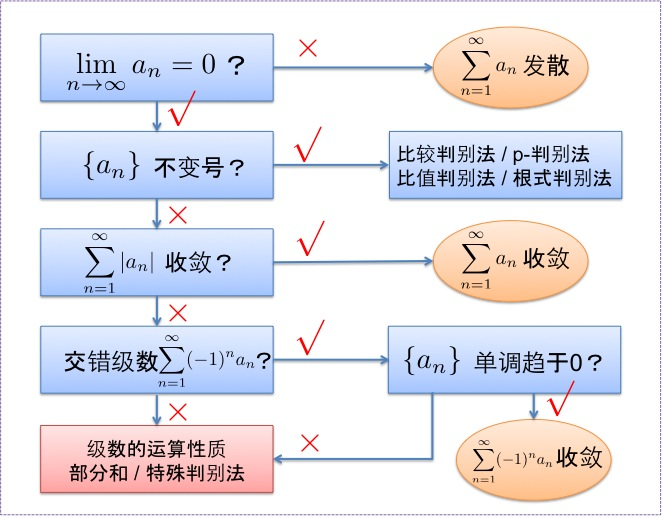
\includegraphics{./images/ch2/seriesCre/010.jpg}}
	
	{\it 级数判敛的大致思路}
\end{center}

{\bf 例:}判断正误:
\begin{enumerate}[(1)]
  \setlength{\itemindent}{1cm}
  \item 若$a_n>0(n=1,2,\ldots)$,则\\
  \centerline{$a_1-a_1+a_2-a_2+a_3-a_3+\ldots $}
  收敛 \hfill ({$\times$})
  \item 若以上$\limn a_n=0$,则以上级数收敛 \hfill
  ({$\surd$})
  \item $\sumn a_n$收敛,$\limn b_n=1\Rightarrow\sumn
  a_nb_n$收敛\ps{本例可以作为{\b 比较判别法不适用于变号级数}的反例} \hfill ({$\times$})
  $${\b \mbox{反例:}a_n=\df{(-1)^n}{\sqrt n},\quad b_n=1+a_n}$$
  \item $\sumn a_n$部分和有界,$\limn b_n=0\Rightarrow\sumn a_nb_n$收敛
  \hfill ({$\times$})
  $$\mbox{反例:}a_n=(-1)^n,\quad b_n=\df{(-1)^n}n$$
  \item 若$\limn\df{a_n}{b_n}=1$,则若$\sumn a_n$绝对收敛,$\sumn b_n$必收敛 \hfill
  ({$\surd$})
  \item $\sumn a_n,\sumn b_n$绝对收敛$\Rightarrow\sumn (a_n+b_n)$绝对收敛 \hfill
  ({$\surd$})
  \item $\sumn a_n,\sumn b_n$条件收敛$\Rightarrow\sumn (a_n+b_n)$条件收敛 \hfill
  ({$\times$})
  \item 若$\sumn a_n^2$收敛,则$\sumn a_n^3$收敛 \hfill
  ({$\surd$})
\end{enumerate}

% {\bf 例:}判断下列级数的敛散性
% \begin{enumerate}[(1)]
%   \setlength{\itemindent}{1cm}
%   
%   \item $\df 1{a+b}+\df 1{2a+b}+\df 1{3a+b}+\ldots\quad (a>0,b>0)$
%   \item $\sumn\df {a_n}{(1+a_1)(1+a_2)\ldots(1+a_n)}\quad(a_n\geq
% 	  0,n\in\mathbb{N})$
% %   \item $\sumn\df{1!+2!+\ldots+n!}{n!}$
%   
% %   \item $\sumn\df{\sqrt{n!}}{(2+\sqrt 1)(2+\sqrt 2)\ldots(2+\sqrt n)}$
%   \item $\sumn\df{\sqrt{n+1}-\sqrt{n}}{n^p}\quad(p>0)$
%   \item $\sumn\df{n^{n+\frac 1{\,n\,}}}{\left(n+\df 1n\right)^n}$\\
% %   {[提示]:}
% %   $$a_n=\df{n^{\df1n}}{\left(1+\df1{n^2}\right)^n}\to1\;(n\to\infty)$$
%   \item $\sumn\df{2^nn!}{n^n}$
%   \item $\sumn n!\left(\df{x}{n}\right)^n\quad (x>0)$\\
% %   {\bf [hint]:} When $x=e$
% %   $$\df{a_{n+1}}{a_n}=\df e{\left(1+\df1n\right)^n}>1.$$
%   \item $\sumn\left[\df 1n-\ln\left(1+\df 1n\right)\right]$
% %   \item $\sumn\df{n^{n+\frac 1{\,n\,}}}{\left(n+\df 1n\right)^n}$
% \end{enumerate}

{\bf 例:}已知级数$\sumn(-1)^n\sqrt n\tan\df1{n^a}$绝对收敛,级数
$\sumn\df{(-1)^n}{n^{3-a}}$条件收敛,则(D)

\quad (A)\;$0<a\leq \df12$\quad(B)\;$1<a<\df52$
\quad (C)\;$1<a<3$\quad(D)\;$\df52<a<3$

{\bf 例:}设$a_n=\cos n\pi\cdot\ln\left(1+\df1{\sqrt n}\right),\;n=1,2,\ldots$,
则(C)
\begin{enumerate}[(A)]
  \setlength{\itemindent}{1cm}
  \item $\sumn a_n$和$\sumn a_n^2$都收敛
  \item $\sumn a_n$和$\sumn a_n^2$都发散
  \item $\sumn a_n$收敛,$\sumn a_n^2$都发散
  \item $\sumn a_n$发散,$\sumn a_n^2$都收敛
\end{enumerate}

{\bf 例:}下列命题中正确的是(D)
\begin{enumerate}[(A)]
  \setlength{\itemindent}{1cm}
  \item 若$u_n<v_n\;(n=1,2,\ldots)$,则$\sumn u_n\leq \sumn v_n$
  \item 若$u_n<v_n\;(n=1,2,\ldots)$,且$\sumn v_n$收敛,则$\sumn u_n$收敛
  \item 若$\limn\df{u_n}{v_n}=1$,且$\sumn v_n$收敛,则$\sumn u_n$收敛
  \item 若$w_n<u_n<v_n\;(n=1,2,\ldots)$,且$\sumn w_n,\sumn v_n$收敛,
  则$\sumn u_n$收敛
\end{enumerate}

{\bf 例:}下列命题中错误的是(D)
\begin{enumerate}[(A)]
  \setlength{\itemindent}{1cm}
  \item 若$\sumn u_n$与$\sumn v_n$均收敛,则$\sumn u_n+v_n$必收敛
  \item 若$\sumn u_n$收敛,$\sumn v_n$发散,则$\sumn u_n+v_n$必发散
  \item 若$\sumn u_n$与$\sumn v_n$均发散,则$\sumn u_n+v_n$未必发散
  \item 若$\sumn u_n+v_n$收敛,则$\sumn u_n$与$\sumn v_n$均收敛
\end{enumerate}


{\bf 例:}对于级数$\sumn(-1)^{n-1}u_n$,其中$u_n>0\;(n=1,2,\ldots)$,
下列命题正确的是(B)
\begin{enumerate}[(A)]
  \setlength{\itemindent}{1cm}
  \item 若$\sumn(-1)^{n-1}u_n$收敛,则必为条件收敛
  \item 若$\sumn u_n$收敛,则$\sumn(-1)^{n-1}u_n$绝对收敛
  \item 若$\sumn u_n$发散,则$\sumn(-1)^{n-1}u_n$发散
  \item 若$\sumn (-1)^{n-1} u_n$收敛,则$\sumn u_n$收敛
\end{enumerate}

{\bf 例:}设$0\leq u_n\leq \df1n$,则下列级数中一定收敛的是(D)

\quad (A)\;$\sumn u_n$\quad(B)\;$\sumn (-1)^n u_n$
\quad (C)\;$\sumn \sqrt{u_n}$\quad(D)\;$\sumn (-1)^nu_n^2$

{\bf 例:}已知$a>0$,则$\sumn(-1)^n\left(1-\cos\df an\right)$(A)

\quad (A)\;绝对收敛\quad(B)\;条件收敛
\quad (C)\;发散\quad(D)\;敛散性与$a$有关

{\bf 例:}级数$\sumn(-1)^n\ln\left(1+\df1n\right)$(C)

\quad (A)\;收敛\quad(B)\;发散
\quad (C)\;条件收敛\quad(D)\;绝对收敛

{\bf 例:}已知$a$为常数,则$\sumn(-1)^n\sin\df{\pi}{\sqrt n}$(D)

\quad (A)\;绝对收敛\quad(B)\;条件收敛
\quad (C)\;发散\quad(D)\;敛散性与$a$有关

{\bf 例:}已知级数$\sumn a_n^2$和$\sumn b_n^2$均收敛,则级数$\sumn a_nb_n$(A)

\quad (A)\;绝对收敛\quad(B)\;条件收敛
\quad (C)\;发散\quad(D)\;敛散性无法判定

{\bf 例:}已知$a_n\geq 0\;(n=1,2,\ldots)$,级数$\sumn a_n^2$收敛,
$\sumn b_n^2$发散,(C) 

\quad (A)\;$\sumn a_nb_n$收敛\quad(B)\;$\sumn a_nb_n$发散
\quad (C)\;$\sumn a_n^3$收敛\quad(D)\;$\sumn b_n^3$发散

{\bf 例:}设$u_n\ne0\;(n=1,2,\ldots)$,且$\limn\df n{u_n}=1$,则
级数$\sumn(-1)^n\left(\df1{u_n}+\df1{u_{n+1}}\right)$(B)

\quad (A)\;绝对收敛\quad(B)\;条件收敛
\quad (C)\;发散\quad(D)\;敛散性无法判定


{\bf 例:}判断下列级数的敛散性
\begin{enumerate}[(1)]
  \setlength{\itemindent}{1cm}
  \item $\sumn\left(1-\df12+\df13-\df14+\ldots+\df{(-1)^{n+1}}n\right)$
%   \hfill({\it 通项不趋于零,发散})
  \item $\df12+\df1{10}+\df1{2^2}+\df1{20}+\ldots+\df1{2^n}+\df1{10n}+\ldots$
  \item $\df 1{a+b}+\df 1{2a+b}+\df 1{3a+b}+\ldots\quad (a>0,b>0)$
  \item $\sumn\df {a_n}{(1+a_1)(1+a_2)\ldots(1+a_n)}\quad(a_n\geq
	  0,n\in\mathbb{N})$
  \item $\sumn\df{\sqrt{n+1}-\sqrt{n}}{n^p}\quad(p>0)$
  \item $\sumn\df{n^{n+\frac 1{\,n\,}}}{\left(n+\df 1n\right)^n}$
  \item $\sumn n!\left(\df{x}{n}\right)^n\quad (x>0)$
  \item $\sumn\left[\df 1n-\ln\left(1+\df 1n\right)\right]$
  \item $\sumn\sin(\pi\sqrt{n^2+a^2})$
  \item $\sum\limits_{n=2}^{\infty}\df{(-1)^n}{\sqrt n+(-1)^n}$
%   \item 
\end{enumerate}

{\bf 例:}证明$\sum\limits_{n=2}^{\infty}\df{(-1)^n}{\sqrt{n+(-1)^n}}$条件收敛

[提示]:与$\sumn\df1{\sqrt{n+1}}$比较易知,该级数不绝对收敛。又
$$S_{2n}=\left(\df1{\sqrt{3}}-\df1{\sqrt{2}}\right)
+\left(\df1{\sqrt{5}}-\df1{\sqrt{4}}\right)+\ldots
+\left(\df1{\sqrt{2n+1}}-\df1{\sqrt{n}}\right)<0,$$
且
$$S_{2n}>\left(\df1{\sqrt{4}}-\df1{\sqrt{2}}\right)
+\left(\df1{\sqrt{6}}-\df1{\sqrt{4}}\right)+\ldots
+\left(\df1{\sqrt{2n+2}}-\df1{\sqrt{n}}\right)
=\df1{\sqrt{2n+2}}-\df1{\sqrt{2}}>-\df1{\sqrt{2}},$$
故$\{S_{2n}\}$收敛。注意到
$$\limn S_{2n+1}=\limn S_{2n}+\limn\df{(-1)^n}{\sqrt{n+(-1)^n}}=\limn S_{2n},$$
由拉链定理,$\{S_n\}$收敛。

综上,原级数条件收敛。

{\bf 例:}设$\sumn u_n$和$\sumn v_n$均为正项级数,证明:
\begin{enumerate}[(1)]
  \setlength{\itemindent}{1cm}
  \item 若$\sumn u_n$收敛,则$\sumn\sqrt{u_nu_{n+1}}$收敛
  \item 若$\sumn\sqrt{u_nu_{n+1}}$收敛,且$\{u_n\}$单调递减,则$\sumn u_n$收敛
  \item 若$\sumn u_n$和$\sumn v_n$均收敛,则$\sumn u_nv_n$收敛
  \item 若$\sumn u_n$收敛,则$\sumn \df{u_n}n$收敛
\end{enumerate}

{\bf 例:}设$u_1=2,\;u_{n+1}=\df12\left(u_n+\df1{u_n}\right),\;(n=1,2,\ldots)$,
证明:级数$\sumn\left(\df{u_n}{u_{n+1}}-1\right)$收敛。

[提示]:易证$u_n\geq 1$且单调递减,故$\limn u_n$存在,且$u_n$均非负,进而
$$0\leq\df{u_n}{u_{n+1}}-1=\df{u_n-u_{n+1}}{u_{n+1}}\leq u_n-u_{n+1}.$$
注意到$\sumn(u_n-u_{n+1})$收敛,由比较判别法,原级数收敛。

{\bf 例:}判断级数$\sum\limits_{n=2}^{\infty}\sin\left(n\pi+\df1{\ln n}\right)$
的敛散性。

[提示]:原级数即为$\sum\limits_{n=2}^{\infty}(-1)^n\sin\df1{\ln n}$。

由$\df1{\ln n}>\df1n$,原级数不绝对收敛。

又$\left(\sin\df1{\ln x}\right)'=-\df1{x(\ln x)^2}\cos\df1{\ln x}<0,$
故通项单调递减,注意到$\limn\sin\df1{\ln n}=0$,
故由Leibniz判别法可知原级数收敛。

综上,原级数条件收敛。

\newpage

\section*{课后作业}
\addcontentsline{toc}{section}{课后作业}

{\bf 【必作题】}

\begin{itemize}
  \item 习题2.1:2,6(1,3),7,9
  \item 证明:$\sqrt[n]n\to 1\,(n\to\infty)$
  \item 习题2.2:1(4,6),2(2,3),3,7,9,11
  \item 习题2.3:4,5
  \item 习题2.4:1(3,4),3,5(2,4),6(1-3),8,9
  \item 习题2.5:2(1,3,6,7,8),3,6,7,8
\end{itemize}

\bigskip

\hrule

\bigskip
\bigskip

{\bf 【思考题】}

\begin{itemize}
  \item 习题2.1:12,15
  \item 习题2.2:8,10,12,17,18
  \item 已知数列$\{a_n\}$单调递增,它的一个子列$\{a_{n_k}\}$收敛于$a$,
  证明:$\limn a_n=a$。
  \item 设$0<a_1<2$,且$(2-a_n)a_{n+1}=1\,(n\in\mathbb{N})$,
  	证明$\{a_n\}$收敛,求其极限。\ps{辅导书(上)-P31-例22}\\
%   {\bf [hint]:} If $a_n=1$, then $a_{n+1}=1$. If $a_n<1$, then $a_{n+1}<1$.
%   If $a_n>2$, then $a_{n+1}<0$, thus $a_{n+2}<\df12$. If $a_n>1$, then 
%   $a_{n+1}>1$. So we have $a_n\in(0,2)$ for sufficient large $n$.\\
%   On the other hand, we have
%   $$a_{n+1}=\df{1-a_{n+1}}{1-a_n}.$$
%   Hence, we can deduce that $a_{n+1}<a_n$, whenever $a_n\in(0,1)$ or 
%   $a_n>1$. So $\{a_n\}$ is mono-increase with upper bound.\\
%   Let $a=\limn a_n$, we can find $a=1$.
  \item 设$x_1=\df 12$,$x_{n+1}=x_n^2+x_n\,(n\in\mathbb{N})$,求
	$$\limn\left(\df 1{x_1+1}+\df 1{x_2+1}+\ldots+\df
	1{x_n+1}\right)$$
%   {\bf [hint]:}$\df1{x_{n+1}}=\df1{x_n}-\df1{x_n+1}$, so we have
%   $$\df1{x_n+1}=\df1{x_n}-\df1{x_{n+1}}$$
%   \item 已知$0<x<1$,数列$\{a_n\}$定义如下:
% 	$$a_1=\df x2,\;a_n=\df x2-\df{a_{n-1}^2}2.$$
% 	证明$\{a_n\}$收敛,并求其极限。
  \item 已知$0<x<1$,数列$\{a_n\}$定义如下:\ps{辅导书(上)-P30-例21}
	$$a_1=\df x2,\;a_n=\df x2+\df{a_{n-1}^2}2.$$
	证明$\{a_n\}$收敛,并求其极限。
% 	\ps{参考辅导书(上)-P30-例21,是不是题目抄错了?应该是$\df x2+\df{a_{n-1}^2}2$}\\
%   {\bf [hint]:} It's easy to find $a_2\in(0,a_1)$. Assume $a_{n}\in
%   (0,a_{n-1})$, then
%   $$a_n=\df x2-\df{a_{n-1}^2}2<\df x2-\df{a_{n}^2}2=a_{n+1}.$$
%   We can find $\limn a_n=\sqrt{x+1}-1$.  
  \item 习题2.3:6,7,8
  \item 习题2.4:10-15,17
  \item 习题2.5:4,10,13
\end{itemize}
% 
\newpage

\section*{习题参考解答}
\addcontentsline{toc}{section}{习题参考解答}

{\bf
习题2.1-2:}(3)设$b_n=0.\underbrace{888\ldots8}_{n\mbox{个}},
\;n=1,2,\ldots$,问:当$n\to\infty$时,是否$b_n\to0.9$?

解:否。事实上,
$$\limn{b_n}=8\cdot\sumn
10^{-n}=0.8\cdot\limn\df{1-10^{-n-1}}{1-10^{-1}}=\df89\ne 0.9.$$

注:{\it 如果用极限的(反面)定义证明,可以令$\e_0=0.01$,则对任意$N\in\mathbb{Z}_+$,
总可以取$n_0=\max\{N,3\}$,使得}
$$|b_n-0.9|>|0.888-0.9|=0.012>0.01.$$
{\it 即证。}

\bigskip

{\bf 习题2.1-6:}用数列极限的定义证明:

\bigskip

(1)$\limn\df{2n+1}{3n+2}=\df23$

证:对任意$\e>0$,令$N=\left[\df1{\e}\right]+1$,则对任意$n>N$,总有
$$\left|\df{2n+1}{3n+2}-\df23\right|=\df1{3(3n+2)}<\df1n<\df1N<\e,$$
由极限的定义,即证。

\bigskip

(3)$\limn\df{\sqrt{n^2+a^2}}n=1$

证:对任意$\e>0$,令$N=\left[\df{a^2}{\e}\right]+1$,则对任意$n>N$,总有
$$\left|\df{\sqrt{n^2+a^2}}n-1\right|
=\df{\sqrt{n^2+a^2}-n}n=\df{a^2}{n(\sqrt{n^2+a^2}+n)}
<\df{a^2}n<\df{a^2}N<\e,$$
由极限的定义,即证。

\bigskip

{\bf 习题2.1-6:}设数列$\{a_n\}$有界,又$\limn b_n=0$,证明:$\limn a_nb_n=0$

证:由$\{a_n\}$有界,存在$M>0$,对任意$n\in\mathbb{Z}_+$,有
$$|a_n|\leq M.$$

对任意$\e>0$,由$\limn b_n=0$,存在$N\in\mathbb{Z}_+$,对任意$n>N$有
$$|b_n-0|<\e,$$
从而当$n>N$时,有
$$|a_nb_n-0|<M\e,$$
由极限的定义,即证。

\bigskip

{\bf 习题2.1-9:}设$\limn a_n=a\ne0$,证明存在$N\in\mathbb{Z}_+$,对任意$n>N$有
$|a_n|>\df{|a|}2.$

证:由$\limn a_n=a\ne0$,对$\e=\df{|a|}2$,存在$N\in\mathbb{Z}_+$,对任意$n>N$有
\ps{$|a|-|a_n|\leq|a_n-a|$}
$$|a_n-a|<\e=\df{|a|}2\quad\Rightarrow\quad |a_n|>\df{|a|}2,$$
即证。

\bigskip

{\bf 习题2.2-2:}试用夹逼定理证明:

(2)$\limn\sqrt[n]{a_1^n+a_2^n+\ldots+a_m^n}=
\max\{a_1,a_2,\ldots,a_m\}$,其中$a_1,a_2,\ldots,a_m$均为正数。

证:设$a=\max\{a_1,a_2,\ldots,a_m\}$,则
$$a<\sqrt[n]{a_1^n+a_2^n+\ldots+a_m^n}\leq\sqrt[n]{m}\cdot a,$$
注意到$\limn\sqrt[n]m=1$,故上式两端当$n\to\infty$时极限均为$a$,由
夹逼定理,即证。

\bigskip

{\bf 补充题:}证明:$\limn\sqrt[n]{n}=1$

证:设$h_n=\sqrt[n]{n}-1$,显然$h_n>0$,从而
$$n=(1+h_n)^n=1+n\cdot h_n+\df{n(n-1)}2h^2_n+\ldots+h_n^n>\df{n(n-1)}2h^2_n,$$
进而可得
$$0<h_n<\sqrt{\df2{n-1}}.$$
注意到$\limn\sqrt{\df2{n-1}}=0$,故由夹逼定理,$\limn h_n=0$,也即$\limn\sqrt[n]{n}=1$.

\bigskip

{\bf 习题2.2-3:}试证明:极限$\limn\sin\df{n\pi}2$不存在。

证:记$a_n=\sin\df{n\pi}2$,则
$$a_{2n}=\sin n\pi\equiv 0,\quad 
a_{4n+1}=\sin\left(2n\pi+\df{\pi}2\right)\equiv 1,$$
由此易知$\{a_n\}$的子数列$\{a_{2n}\}$和$\{a_{4n+1}\}$分别收敛到$0$和$1$,
从而由子数列收敛与数列收敛的关系,可知数列$\{a_n\}$发散,即证。

\bigskip

{\bf 习题2.2-11:}证明:若$a_1+a_2+\ldots+a_k=0$,则
$$\limn\left(a_1\sqrt{n+1}+a_2\sqrt{n+2}+\ldots
+a_k\sqrt{n+k}\right)=0.$$

证:
\begin{align}
	\mbox{原式}
	&=\limn\left[a_1\sqrt{n+1}+a_2\sqrt{n+2}+\ldots+a_k\sqrt{n+k}
	-(a_1+a_2+\ldots+a_k)\sqrt n\right]\notag\\
	&=\limn\left[a_1(\sqrt{n+1}-\sqrt n)+a_2(\sqrt{n+2}-\sqrt
	n)+\ldots+a_k(\sqrt{n+k} -\sqrt n)\right]\notag\\
	&=a_1\limn(\sqrt{n+1}-\sqrt n)+a_2\limn(\sqrt{n+2}-\sqrt
	n)+\ldots+a_k\limn(\sqrt{n+k} -\sqrt n).\notag
\end{align}
注意到对任意$i\in\{1,2,\ldots,k\}$,
$$\limn(\sqrt{n+i}-\sqrt n)=\limn\df{i}{\sqrt{n+i}+\sqrt n}=0,$$
故$\mbox{原式}=0$,即证。

% 
% $$\df1{x^3(1+x^4)}=\df{Ax^2+Bx+C}{x^3}+\df{Dx^3+Ex^2+Fx+G}{1+x^4}$$

\newpage

\section*{附加讨论题}
\addcontentsline{toc}{section}{附加讨论题}

{\bf 例:}已知数列$\{a_n\}$单调递增,它的一个子列$\{a_{n_k}\}$收敛于$a$,
  证明:$\limn a_n=a$。
  
  {\bf 证1:} 由$a_{n_k}\to a(k\to\infty)$,对$\forall\e>0$,$\exists K$,
  $\forall k>K$,$|a_{n_k}-a|<\e$,或
  $$a_{n_k}\in U(a,\e).$$
  令$N=n_{[K]+1}$,则对$\forall n>N$,注意到$\{a_n\}$单调递增,故一定
  $\exists k>K$,使得$a_na_{n_k}\leq n<a_{n_{k+1}}$,进而
  $$a_n\in[a_{n_k},a_{n_{k+1}})\subset U(a,\e),$$
  即证。\\
  {\bf 证2:} 由$\{a_n\}$单调递增,对$\forall n\in\mathbb{Z}_+$,
  $\exists k\in\mathbb{Z}_+$,使得
  $$a_{n_k}\leq n<a_{n_{k+1}}.$$
  定义两个数列
  $$a_n^{(1)}=a_{n_k},\;\mbox{若}a_{n_k}\leq n<a_{n_{k+1}},$$
  $$a_n^{(2)}=a_{n_{k+1}},\;\mbox{若}a_{n_k}\leq n<a_{n_{k+1}},$$
  则
  $$a_n^{(1)}\leq a_n<a_n^{(2)}.$$
  注意到$\{a_n^{(1)}\},\{a_n^{(2)}\}$的取值范围和$\{a_{n_k}\}$完全相同,
  且均单调递增,故易知其极限均为$a$。进而,有夹逼定理可知$a_n\to a(n\to\infty)$

\bigskip

{\bf 命题:}若$\{a_n\}$有界,且$\{a_n-a_{n-1}\}$收敛于$0$,则$\{a_n\}$收敛。

{\bf 反例:}

(1)$\sin\sqrt n$

(2)$\left\{\left(\sum\limits_{k=1}^n\df1k\right)\mod
2-1\right\}(-1)^{\left[\frac12{\sum\limits_{k=1}^n\frac1k}\right]}$

\bigskip

{\bf 例:}已知$0<x<1$,数列$\{a_n\}$定义如下:
$$a_1=\df x2,\;a_n=\df x2-\df{a_{n-1}^2}2.$$
证明$\{a_n\}$收敛,并求其极限。

{\bf 证}: 若极限存在,易求得$\limn a_n=1+\sqrt{1+x}$。以下证明$\{a_n\}$收敛。

显然$x_n\in\left(0,\df x2\right),(n\in\mathbb Z_+)$。由递推公式可得

% 显然,$x_n<\df x2\;(n\in\mathbb{Z}_+)$。
% \begin{align}
% 	a_n-a_{n-1}&=-\df12(a_{n-1}-a_{n-2})(a_{n-1}+a_{n-2})\notag\\
% 	&=\left(-\df12\right)^2(a_{n-2}-a_{n-3})(a_{n-2}+a_{n-3})(a_{n-1}+a_{n-2})\notag\\
% 	&=\ldots=\left(-\df12\right)^{n-2}(a_2-a_1)(a_2+a_1)\ldots
% 	(a_{n-2}+a_{n-3})(a_{n-1}+a_{n-2})\notag
% \end{align}
% 注意到对任意$n\in\mathbb{Z}_+$
% $$a_n+a_{n-1}=\df{1+x}2-\df12(a_n-1)^2<\df{1+x}2<1,$$
% 故有
% $$|a_n-a_{n-1}|<|a_2-a_1|\left(\df{1+x}4\right)^{n-2}\to0,
% \;(n\to\infty)$$

$$a_n-a_{n-1}=-\df12(a_{n-1}-a_{n-2})(a_{n-1}+a_{n-2}),$$
由此可知若$a_{n-1}>a_{n-2}$,则$a_n<a_{n-1}$。又
$$a_n+a_{n-1}=\df{1+x}2-\df12(a_n-1)^2<\df{1+x}2<1,$$
故
$$|a_n-a_{n-1}|<\df12|a_{n-1}-a_{n-2}|.$$
从而,若$a_{n-1}>a_{n-2}$,则必有$a_{n-2}<a_n<a_{n-1}$,进而
可以证明$a_n<a_{n+1}<a_{n-1}$,也即$[a_n,a_{n+1}]\subset[a_{n-2},a_{n-1}]$。
注意到$x_2<x_1$,故可以断言$\{a_n\}$的偶子列和奇子列分别是单调递增
和单调递减的,从而区间序列$\{[a_{2n},a_{2n-1}]\}$构成了一个区间套,也即
$$[a_{2n+2},a_{2n+1}]\subset[a_{2n},a_{2n-1}],\;(n\in\mathbb Z_+).$$

另一方面,由
\begin{align}
	a_n-a_{n-1}&=-\df12(a_{n-1}-a_{n-2})(a_{n-1}+a_{n-2})\notag\\
	&=\left(-\df12\right)^2(a_{n-2}-a_{n-3})(a_{n-2}+a_{n-3})(a_{n-1}+a_{n-2})\notag\\
	&=\ldots=\left(-\df12\right)^{n-2}(a_2-a_1)(a_2+a_1)\ldots
	(a_{n-2}+a_{n-3})(a_{n-1}+a_{n-2}),\notag
\end{align}
可得
$$|a_n-a_{n-1}|<|a_2-a_1|\left(\df{1+x}4\right)^{n-2}\to0,
\;(n\to\infty),$$
从而必有$\limn(a_n-a_{n-1})=0$,进而$\limn(a_{2n}-a_{2n-1})=0$。

综上,区间序列$\{[a_{2n},a_{2n-1}]\}$满足区间套定理(习题2.2-12)条件,
从而$\{a_{2n}\}$和$\{a_{2n-1}\}$收敛于相同的极限,由拉链定理,$\{a_n\}$收敛。

\bigskip

{\bf 例:}设$\limn a_n=a>0$,判断级数$\sumn\left(\df{a}{a_n}\right)^n$
的敛散性

[提示]:由条件不能判定!

(1)若$a_n=a$,显然级数发散。

(2)设$a_n=\df{1+\sqrt n}{\sqrt n}\to1=a(n\to\infty)$,则
$$\sumn\left(\df{a}{a_n}\right)^n=\sumn\left(\df{\sqrt n}
{1+\sqrt n}\right)^n,$$
由对数判别法
$$-\limn\df{\ln \left(\df{\sqrt n}{1+\sqrt n}\right)^n}
{\ln n}=\limn\df{n[\ln(\sqrt n+1)-\ln\sqrt n]}{\ln n}
=\limn\df{\sqrt n}{\ln n}=+\infty>1,$$
故级数收敛。
